\documentclass[Journal, letterpaper, DoubleSpace, InsideFigs]{ascelike-new}
% For arXiv:
% \documentclass[NewProceedindgs, NoLineNumbers, SectionNumbers, letterpaper, SingleSpace, InsideFigs]{ascelike-new}

%\usepackage{etex}
%\newcommand{\num}{6{} }

%\raggedbottom

%geometry (sets margin) and other useful packages
% \usepackage{geometry}
% \geometry{top=1.2in, left=1in,right=1in,bottom=1in,headsep=6pt}
\usepackage{graphicx,booktabs, calc}

%=== GRAPHICS PATH ===========
\graphicspath{{./figures/}}
% Marginpar width
%Marginpar width
% \newcommand{\pts}[1]{\marginpar{ \small\hspace{0pt} \textit{[#1]} } }
% \setlength{\marginparwidth}{.5in}
%\reversemarginpar
%\setlength{\marginparsep}{.02in}

%% Fonts
% \usepackage{fourier}
% \usepackage[T1]{pbsi}
%\usepackage[utf8]{inputenc}
\usepackage[T1]{fontenc}
\usepackage{lmodern}
%\usepackage{minted}
\usepackage[figurename=Fig.,labelfont=bf,labelsep=period]{caption}
\usepackage{subcaption}
\usepackage{amsmath}
\usepackage{newtxtext,newtxmath}
\usepackage[colorlinks=true,citecolor=red,linkcolor=black]{hyperref}
\usepackage[table]{xcolor}


% %% Captions
% \usepackage{caption}
% \captionsetup{
%   labelsep=quad,
%   justification=raggedright,
%   labelfont=sc
% }

%AMS-TeX packages
%\usepackage{amssymb,amsmath,amsthm}
\usepackage{bm}
%\usepackage[mathscr]{eucal}
%\usepackage{colortbl}
 
 
\usepackage{enumerate}
\usepackage{siunitx}

\usepackage{multirow,array,multicol}
%%%%%%%%%%%%%%%%%%%%%%%%%%%%%%%%%%%%%%%%%%%%%%%%%%%
%%%%%%%%%%%%%%%%%%%%%%%%%%%%%%%%%%%%%%%%%%%%%%%%%%%
\NameTag{Oke, \today}

\begin{document}
% ALL CAPS TITLE REQUIRED
\title{Predicting tree failure likelihood for utility risk mitigation via artificial intelligence}
\author[1]{Jimi Oke}
\author[1]{Nasko Apostolov}
\author[2]{Ryan Suttle}
\author[1]{Sanjay Arwade}
\author[2]{Brian Kane}

\affil[1]{Department of Civil and Environmental Engineering, University of Massachusetts Amherst, MA 01003, USA} %. Email: author.one@umass.edu}
\affil[2]{Department of Environmental Conservation, University of Massachusetts Amherst, MA 01003, USA}

\maketitle

\begin{abstract}
  Critical to the resilience of utility power lines, tree failure assessments have historically been performed via
  manual and visual inspections.  In this paper, we develop a convolutional neural network (CNN) to predict tree failure
  likelihood categories (\textit{Probable}, \textit{Possible}, \textit{Improbable}) under four classification scenarios.
  Starting with an original set of 505 expert-labeled images, we performed preprocessing and augmentation tasks to
  increase the number of samples by a factor of 5. We optimized several hyperparameters in the CNN and then trained and assessed its performance via cross-validation
  for three different image resolutions under all four scenarios. The CNN produced a validation accuracy of at least 0.94
  ($\hat\sigma = 0.1)$ in the best-performing, yet hypothetical scenario as it excludes one of the categories.  The
  second-best performing scenario, which includes all categories and therefore more practical, resulted in a validation
  accuracy of 0.92 ($\hat\sigma = 0.1$). Thus, via this novel framework, we demonstrate the potential of artificial
  intelligence to automate and consequently reduce the costs of tree failure likelihood assessments, thereby promoting
  sustainable infrastructure.
\end{abstract}

\section{Introduction}
Despite extensive efforts by utilities to prevent them, contacts between tree parts and power lines cause outages that annually result in tens of billions of dollars in economic costs throughout the United States.  Presently, the identification of potential contact between trees and power lines is labor intensive and time-consuming.  This paper describes an artificial intelligence and machine learning approach that automatically classifies trees, using only a single photograph and with a high degree of accuracy, into categories used by utility arborists to describe the likelihood of tree failure: probable, possible, and improbable.  This preliminary study demonstrates the possible efficacy of AI approaches to tree risk assessment and, following further development of the approach, has the potential to reduce power outages and utility costs by allowing utilities to more effectively target their pruning and mitigation efforts.  

Contact between tree parts and power lines can take three forms: tree branches can grow into lines; branches can fail and fall onto lines; whole-tree failure can occur due to uprooting or trunk failure.  A study in Connecticut, USA provides some context for the amount of economic disruption, documenting annual disruptions of \$8.3 billion between 2005 and 2015 \cite{graziano2020wider}.  That extremely high cost occurred despite extensive efforts on the part of utilities to mitigate conflicts between trees and power lines through active and aggressive pruning programs that, on their own cost billions of dollars annually \cite{guggenmoos2003effects}.  

Despite its high cost, pruning trees to maintain clearance from power lines is an effective way to reduce outages due to so-called ``preventable'' contacts between trees and power lines.  For example, in Massachusetts, USA, where tree failure was responsible for 40\% of preventable tree-caused outages, pruning was able to improve reliability by 20\% to 30\% \cite{simpson1996treecaused}; similar results were found in a study conducted in Connecticut \cite{parent2019analysis}. The efficacy of pruning has also been shown in a study of two states in the Gulf Coast region of the USA that showed wind-induced power outage prediction models becoming less uncertain when pruning was included in the model \cite{nateghi2014power}.

Even effective pruning cannot, however, completely eliminate tree-caused outages. Failure of trees outside the right-of-way can still impact the lines and cause outages \cite{guggenmoos2003effects}. The proportion of outages caused by failure of trees outside the right-of-way has not been rigorously quantified. \citeN{guggenmoos2011treerelated} estimated that 95\% of tree-caused outages in the Pacific Northwest region of the USA, were due to tree failure, and \citeN{wismer2018targeted} reported approximately 25\% of interruptions in Illinois, USA, were caused by trees that uprooted or broke in the stem. 

Predicting the likelihood of failure is an inexact science, but tree risk assessment best management practices have been developed \cite{smiley2017best,goodfellow2020best}. Estimating tree risk includes assessing the likelihood of tree failure, the likelihood of impact of the failed tree (or tree part) on a target, and the severity of consequences of the impact. The likelihood of failure depends on the anticipated loads on the tree and its load-bearing capacity. The likelihood of impact depends on proximity to the target (the lines, poles, and other hardware---``infrastructure''---in the case of utility tree risk assessment), the target’s occupancy rate (which is constant for utility lines) and whether the target is sheltered, for example by neighboring trees. Severity of consequences depends on the damage done to the infrastructure---which, in turn, is partially related to the size of the tree or tree part that fails, and how much momentum it has when it impacts the infrastructure---and, more importantly in some cases, the economic costs and disruption associated with electrical outages.

Individual tree risk assessment can be costly because of the time it requires. In some situations, a less time-consuming assessment may be justified to reduce costs, i.e.\ a ``Level 1'' assessment  \cite{smiley2017best}. Studies in Rhode Island, USA \cite{rooney2005reliability} and Florida, USA \cite{koeser2016frequency} have shown that, compared to more time-consuming risk assessments, Level 1 risk assessments successfully identified trees with a higher degree of risk--precisely the trees that arborists prioritize for risk mitigation. The utility of Level 1 assessments demonstrated in these studies suggests that artificial intelligence (AI) tools may be an effective way to reduce the cost of tree risk assessment while still identifying high risk trees.

The method described in the paper uses convolutional neural networks (CNN) to classify images of trees among three categories of failure likelihood: probable, possible, and improbable.  The data used for training, testing and illustration of the method consists of 505 tree images that have been classified by the authors according to best management practices used by utility arborists \cite{goodfellow2020best}. 

The remainder of the paper provides a brief history and background of AI and its use in infrastructure risk assessment and tree identification (section 2); describes the methods used to train and validate a novel CNN to categorize likelihood of tree failure (section 3); and presents and discusses the output of the novel CNN (sections 4 and 5). The goal is to further demonstrate an innovative automated approach to tree risk assessment using an AI tool that can be readily deployed for use in various locations and also continually improved through subsequent training on new datasets.



\section{Background}

AI-based image analysis is relatively widely used, even in engineering applications, such as earthquake risk assessment \cite{jiao2020artificial,salehi2018emerging} and structural health monitoring \cite{spencer2019advances,wang2019novel}. Neural networks, which comprise a major category of AI frameworks, have been widely applied in the field of earthquake risk assessment (an excellent review is provided by \citeN{xie2020promise}), but the authors are not aware of attempts to operate directly on, for example, building images in the absence of technical structural data to predict seismic risk.  Neural networks have also been used to interrogate remote sensing data of the landscape to assess landslide risk \cite{su2020deep}.
A few recent efforts have demonstrated the potential for AI-based tree recognition from drone imagery \cite{santos2019assessment,egli2020cnnbased}. Furthermore, an application of a convolutional neural network (CNN) to tree species identification using was recently demonstrated by \citeN{fricker2019convolutional}. 
Yet, AI has yet to be applied to the problem of tree-utility line risk assessment---one that is complicated by the very large number of tree species to be considered, seasonal variation in tree appearance and associated risk and local meteorological conditions. 


The groundbreaking study of \citeN{hubel1959receptive} showed that visual perception in cats was a result of the
activation or inhibition of groups of cells in the visual cortex known as ``receptive fields.''  Further, they attempted
to map the cortical architecture in cats and monkeys \cite{hubel1962receptive,hubel1965receptive,hubel1968receptive}.
Subsequent attempts were then made to model neural networks that could be trained to automatically recognize visual patterns with modest performance \cite{rosenblatt1962principles,kabrisky1966proposed,giebel1971feature,fukushima1975cognitron}. However, the breakthrough came with the ``neocognitron'' \cite{fukushima1980neocognitron}, which
was a self-learning neural network for pattern recognition that was robust to changes in position and shape distortion, a problem that plagued earlier efforts, including the ``cognitron'' also proposed by \citeN{fukushima1975cognitron}. %proposed a few years earlier.

A few notable efforts demonstrated the neural networks for handwritten digit recognition
\cite{fukushima1988neocognitron,denker1988neural}, but these required significant preprocessing and feature
extraction. \citeN{lecun1989handwritten} soon afterward introduced a multilayer neural network that mapped a feature in each neuron (representing a ``local receptive field'') via convolution. This network could also be trained by backpropagation like other existing neural networks and featured pooling operations for better distortion and
translation invariance. Further developments from this milestone yielded the LeNet-5 convolutional neural network which attained accuracy levels that rendered it commercially viable.

The big data revolution coupled with technological advancements that have made it possible to capture and store high resolution images have raised challenges that continue to be surmounted with successively high-performing
architectures. Over the past decade, some of these efforts resulted in significant breakthroughs in performance. AlexNet \cite{krizhevsky2012imageneta}, with 5 convolutional layers and 3 dense layers---one of the largest CNNs of its time, won the ILSVRC-2012\footnote{ImageNet Large Scale Visual Recognition Challenge; held annually from 2010 through 2017.} competition with a top-5 error rate of 15.3\% and served as a landmark in the Deep Learning subdomain. \citeN{zeiler2014visualizing} then introduced ZFNet, besting the performance of AlexNet, and pioneered visualization techniques that were foundational for model inference and interpretability.  In the same year, GoogLeNet, a 22-layer network, was proposed \cite{szegedy2014going}, featuring the novel ``Inception module,'' which allowed for efficiency and accuracy in a very deep network. Subsequent improvements have been proposed to the original inception framework \cite{szegedy2015rethinking,szegedy2016inceptionv4}.  VGGNet \cite{simonyan2015very} also pushed the boundaries of depth with up 19 layers, achieving state-of-the-art performance at ILSVRC-2014. Finally, ResNet \cite{he2015deep} addressed the accuracy degradation problem that arises with increasing depth in a network by successively fitting smaller sets of layers to the residual and employing skip connections. With these innovations, an unprecedented level of depth was achieved. Implementations with with 34, 50, 101 and 152 layers were demonstrated. ResNet-152 won first place in ILSVRC-2015.

Along with these developments in their architectures, CNNs have demonstrated viability for applications ranging from image classification, object and text detection to document tracking, labeling, speech, among several other related
fields \cite{gu2018recent}. 
In this study, we show that a relatively simple CNN architecture coupled with state-of-the-art approaches for model training and regularization is capable of efficiently and effectively predicting tree failure classes.
%\hl{Paragraph on applications to be completed---with particular attention paid to tree-related efforts.}


\section{Data and Methods}
\subsection{Image data description}
The training dataset consisted of 505 images, each having an original size of $4032\times3024$ pixels.   Images were captured over a single field season in Massachusetts, USA, between May and September 2020 to limit any potential influence of changes in tree appearance due to seasonal leaf senescence on image processing.  ESRI ArcMaps was used to randomly distribute sampling sites across the state.  Field assessments of trees to classify likelihood of failure followed the “Level 1” methods outlined in the second edition of the International Society of Arboriculture’s (ISA) Tree Risk Assessment Best Management Practices \cite{smiley2017best} and ISA’s Utility Tree Risk Assessment Best Management Practices \cite{goodfellow2020best}.  This method is commonly used to assess trees in the United States.  A Level 1 assessment was selected for this study because: (1) individual risk assessments may be prohibitively expensive at higher orders, i.e. Level 2 or Level 3 \cite{smiley2017best}, given the hundreds of thousands of trees utilities must manage across territory areas;  (2) utility right-of-way (ROW) easements may not allow utility inspectors full access to trees in practical application of higher order risk assessment procedure if the trees are beyond the edge of the ROW \cite{goodfellow2020best}; and (3) studies have shown reasonable efficacy of limited basic visual assessment techniques in identifying more severe tree defects \cite{rooney2005reliability,koeser2016frequency} leading to greater likelihood of failure ratings.  The four categories of likelihood of tree failure, which are always considered in a stated time frame, are defined as follows \cite{smiley2017best}:
\begin{itemize}
\item \textit{Improbable}: failure unlikely either during normal or extreme weather conditions;
\item \textit{Possible}: failure expected under extreme weather conditions; but unlikely during normal weather conditions;
\item \textit{Probable}: failure expected under normal weather conditions within a given time frame;
\item \textit{Imminent}: failure has started or is most likely to occur in the near future, even if there is no significant wind or increased load. This is a rare occurrence for a risk assessor to encounter, and may require immediate action to protect targets from impact.
\end{itemize}
In this study, only images of trees assigned to the likelihood of failure categories of \textit{Improbable}, \textit{Possible} and \textit{Probable} were included in modeling. Images of \textit{Imminent} trees were excluded due to their rarity. Typical examples are shown for each category in \autoref{fig:raw_images}.  In the original set of training images, the class distribution is given in \autoref{tab:classdist}.

\begin{figure}[ht]
  \centering
  \begin{subfigure}[t]{.325\linewidth}\centering
    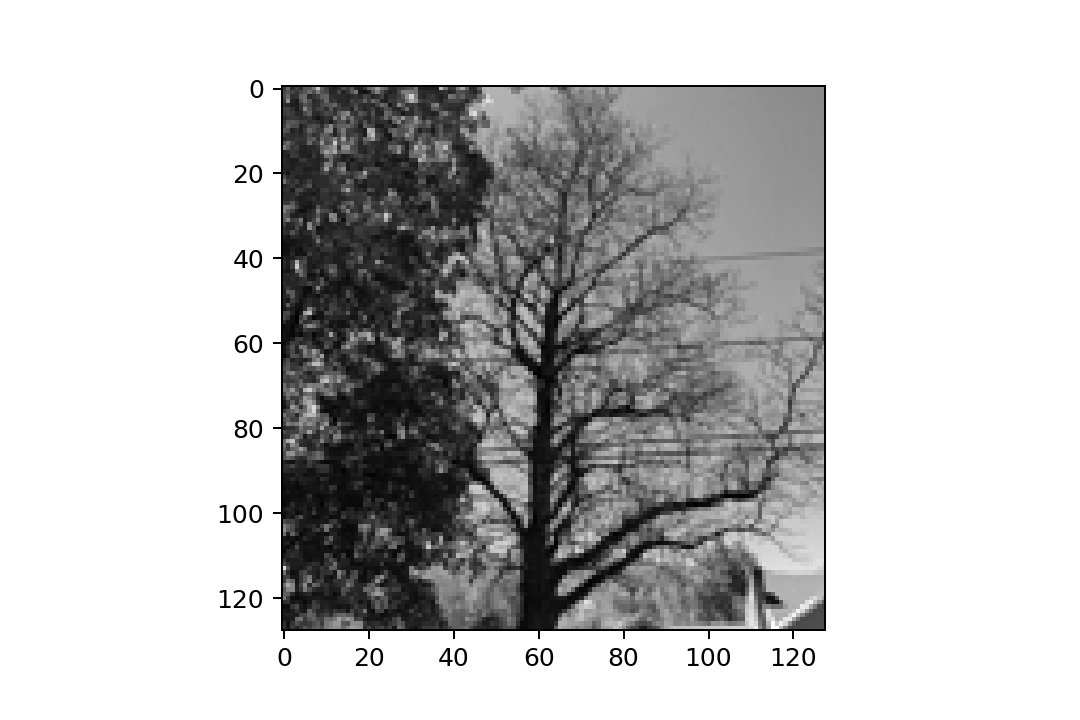
\includegraphics[width=\textwidth,keepaspectratio=true,angle=-90]{probable-example-1} %probable_standing dead.JPG

    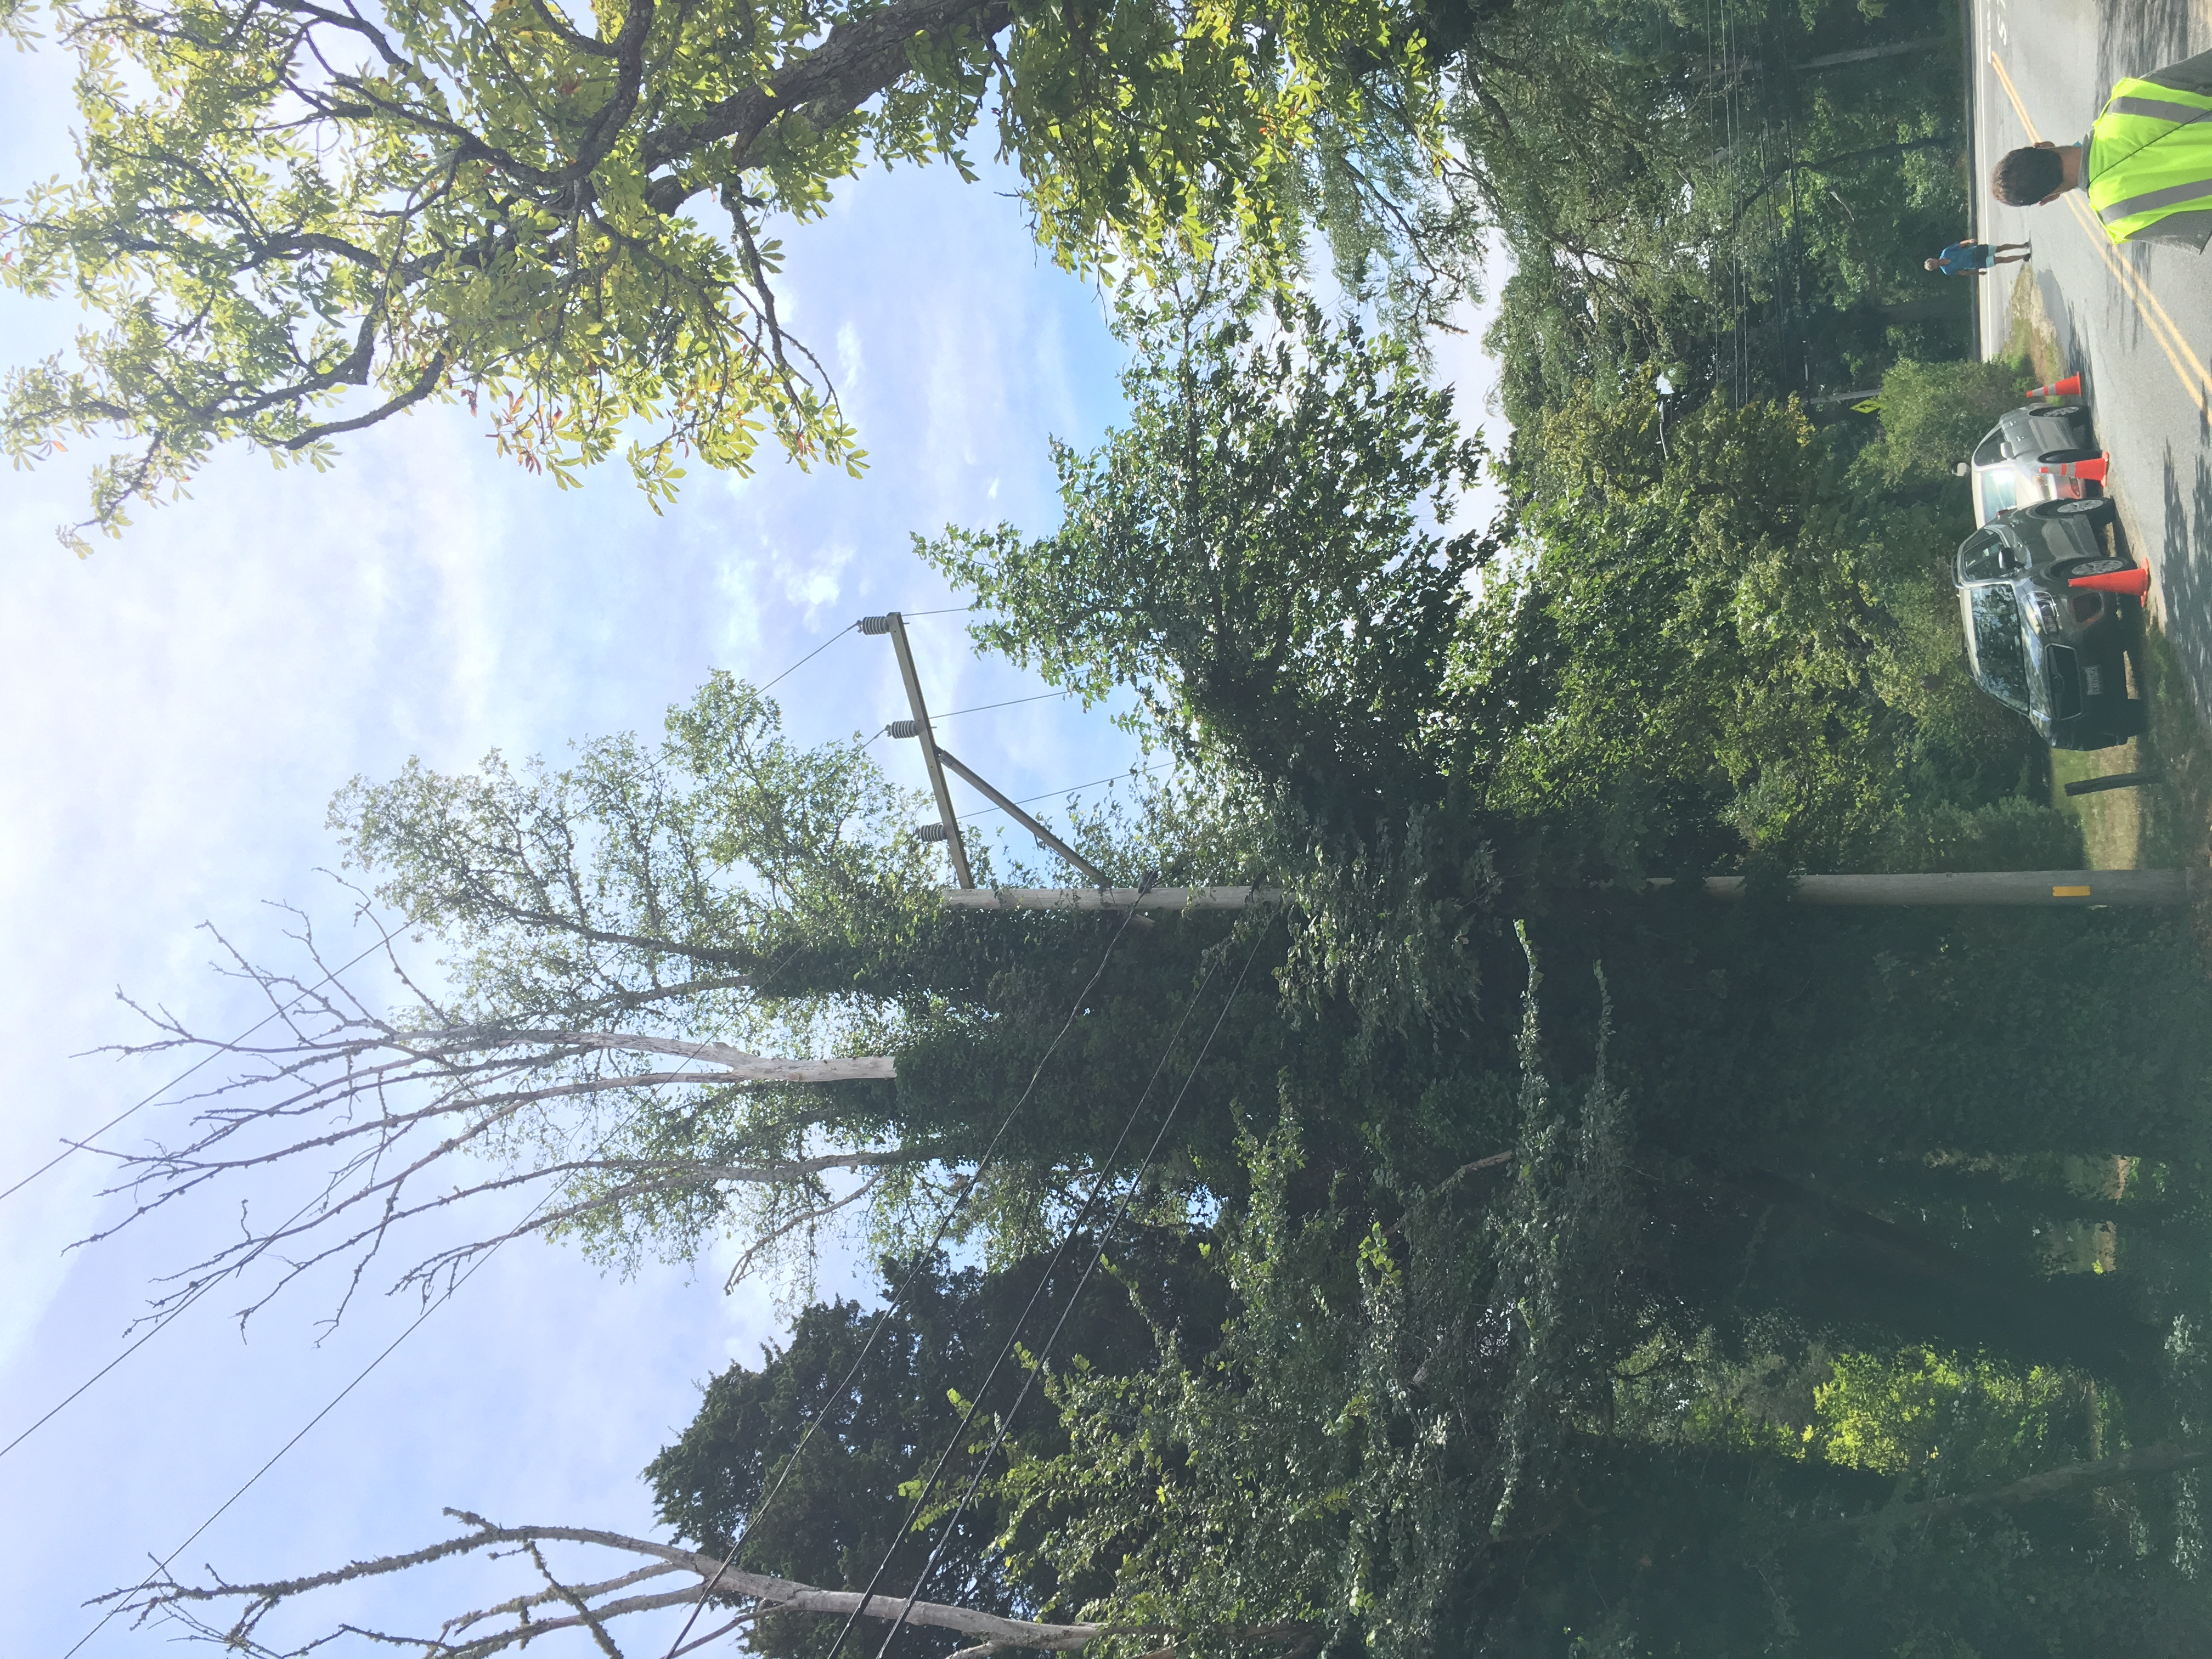
\includegraphics[width=\textwidth,keepaspectratio=true,angle=-90]{probable-example-2} %Probable (deadwood above line hieght, vine)
    \caption{Probable}
  \end{subfigure}
  \begin{subfigure}[t]{.325\linewidth}\centering
    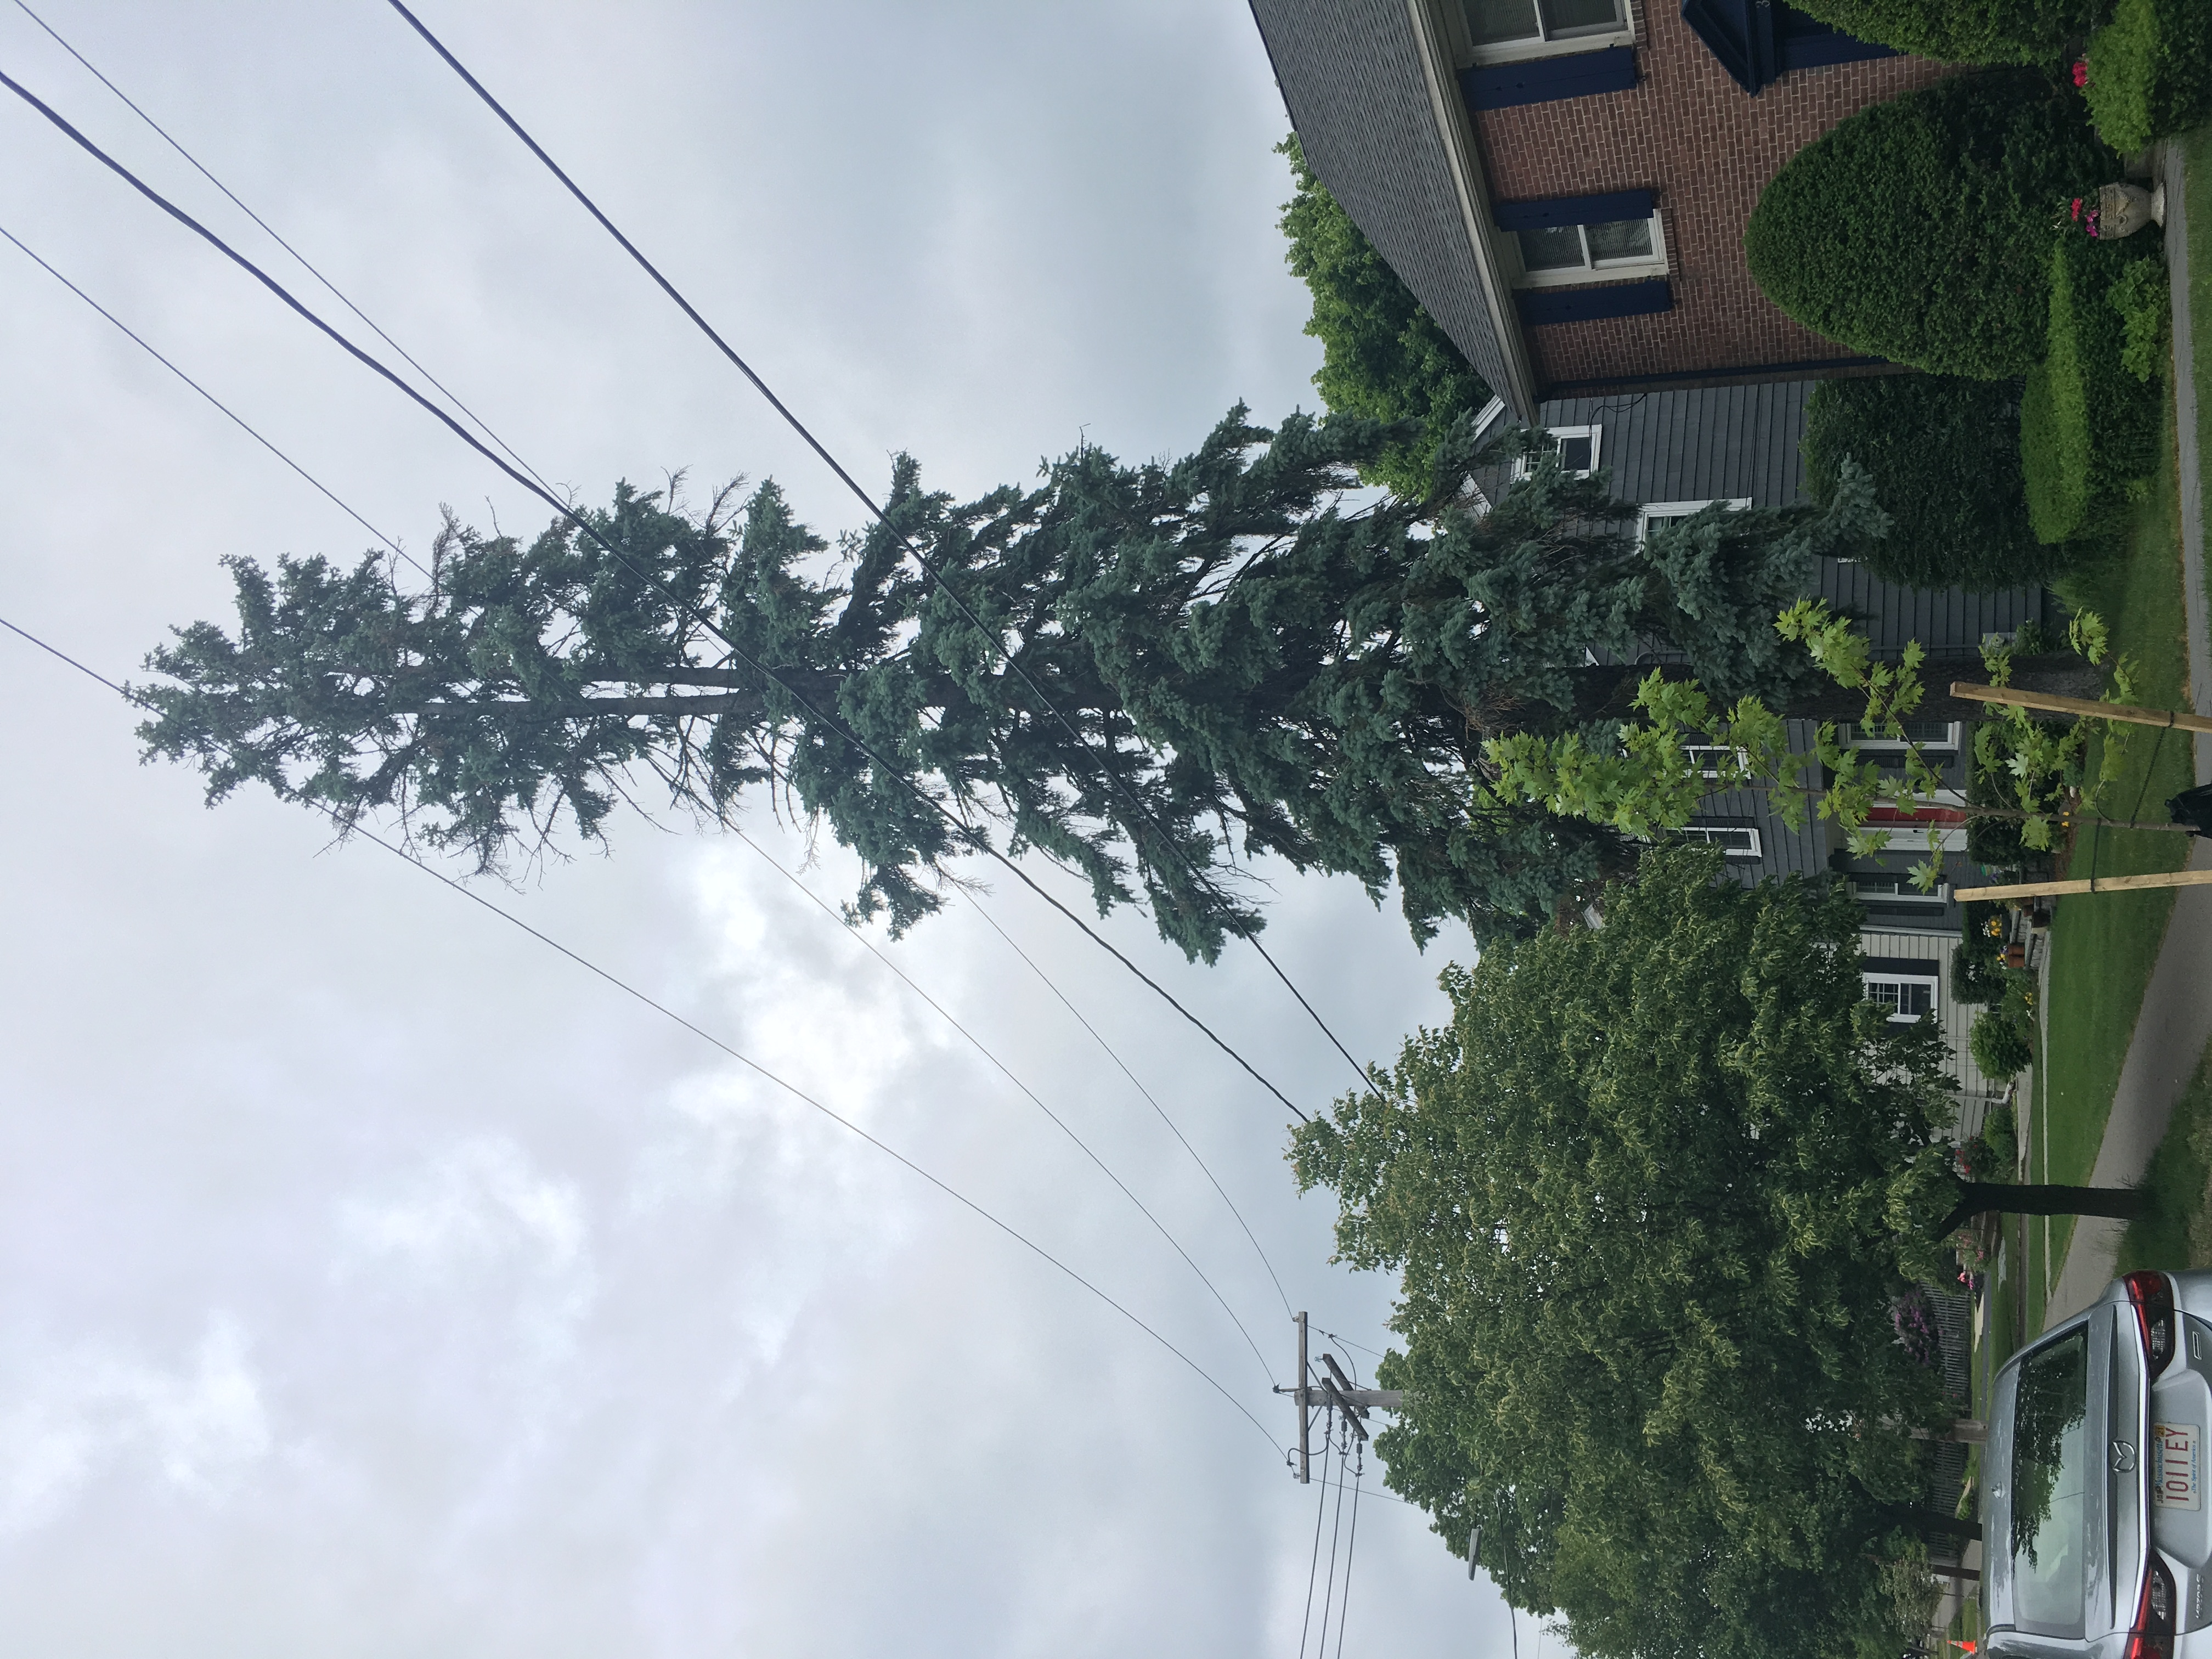
\includegraphics[width=\textwidth,keepaspectratio=true,angle=-90]{possible-example-1} % Possible (spruce, codominant and dieback)

    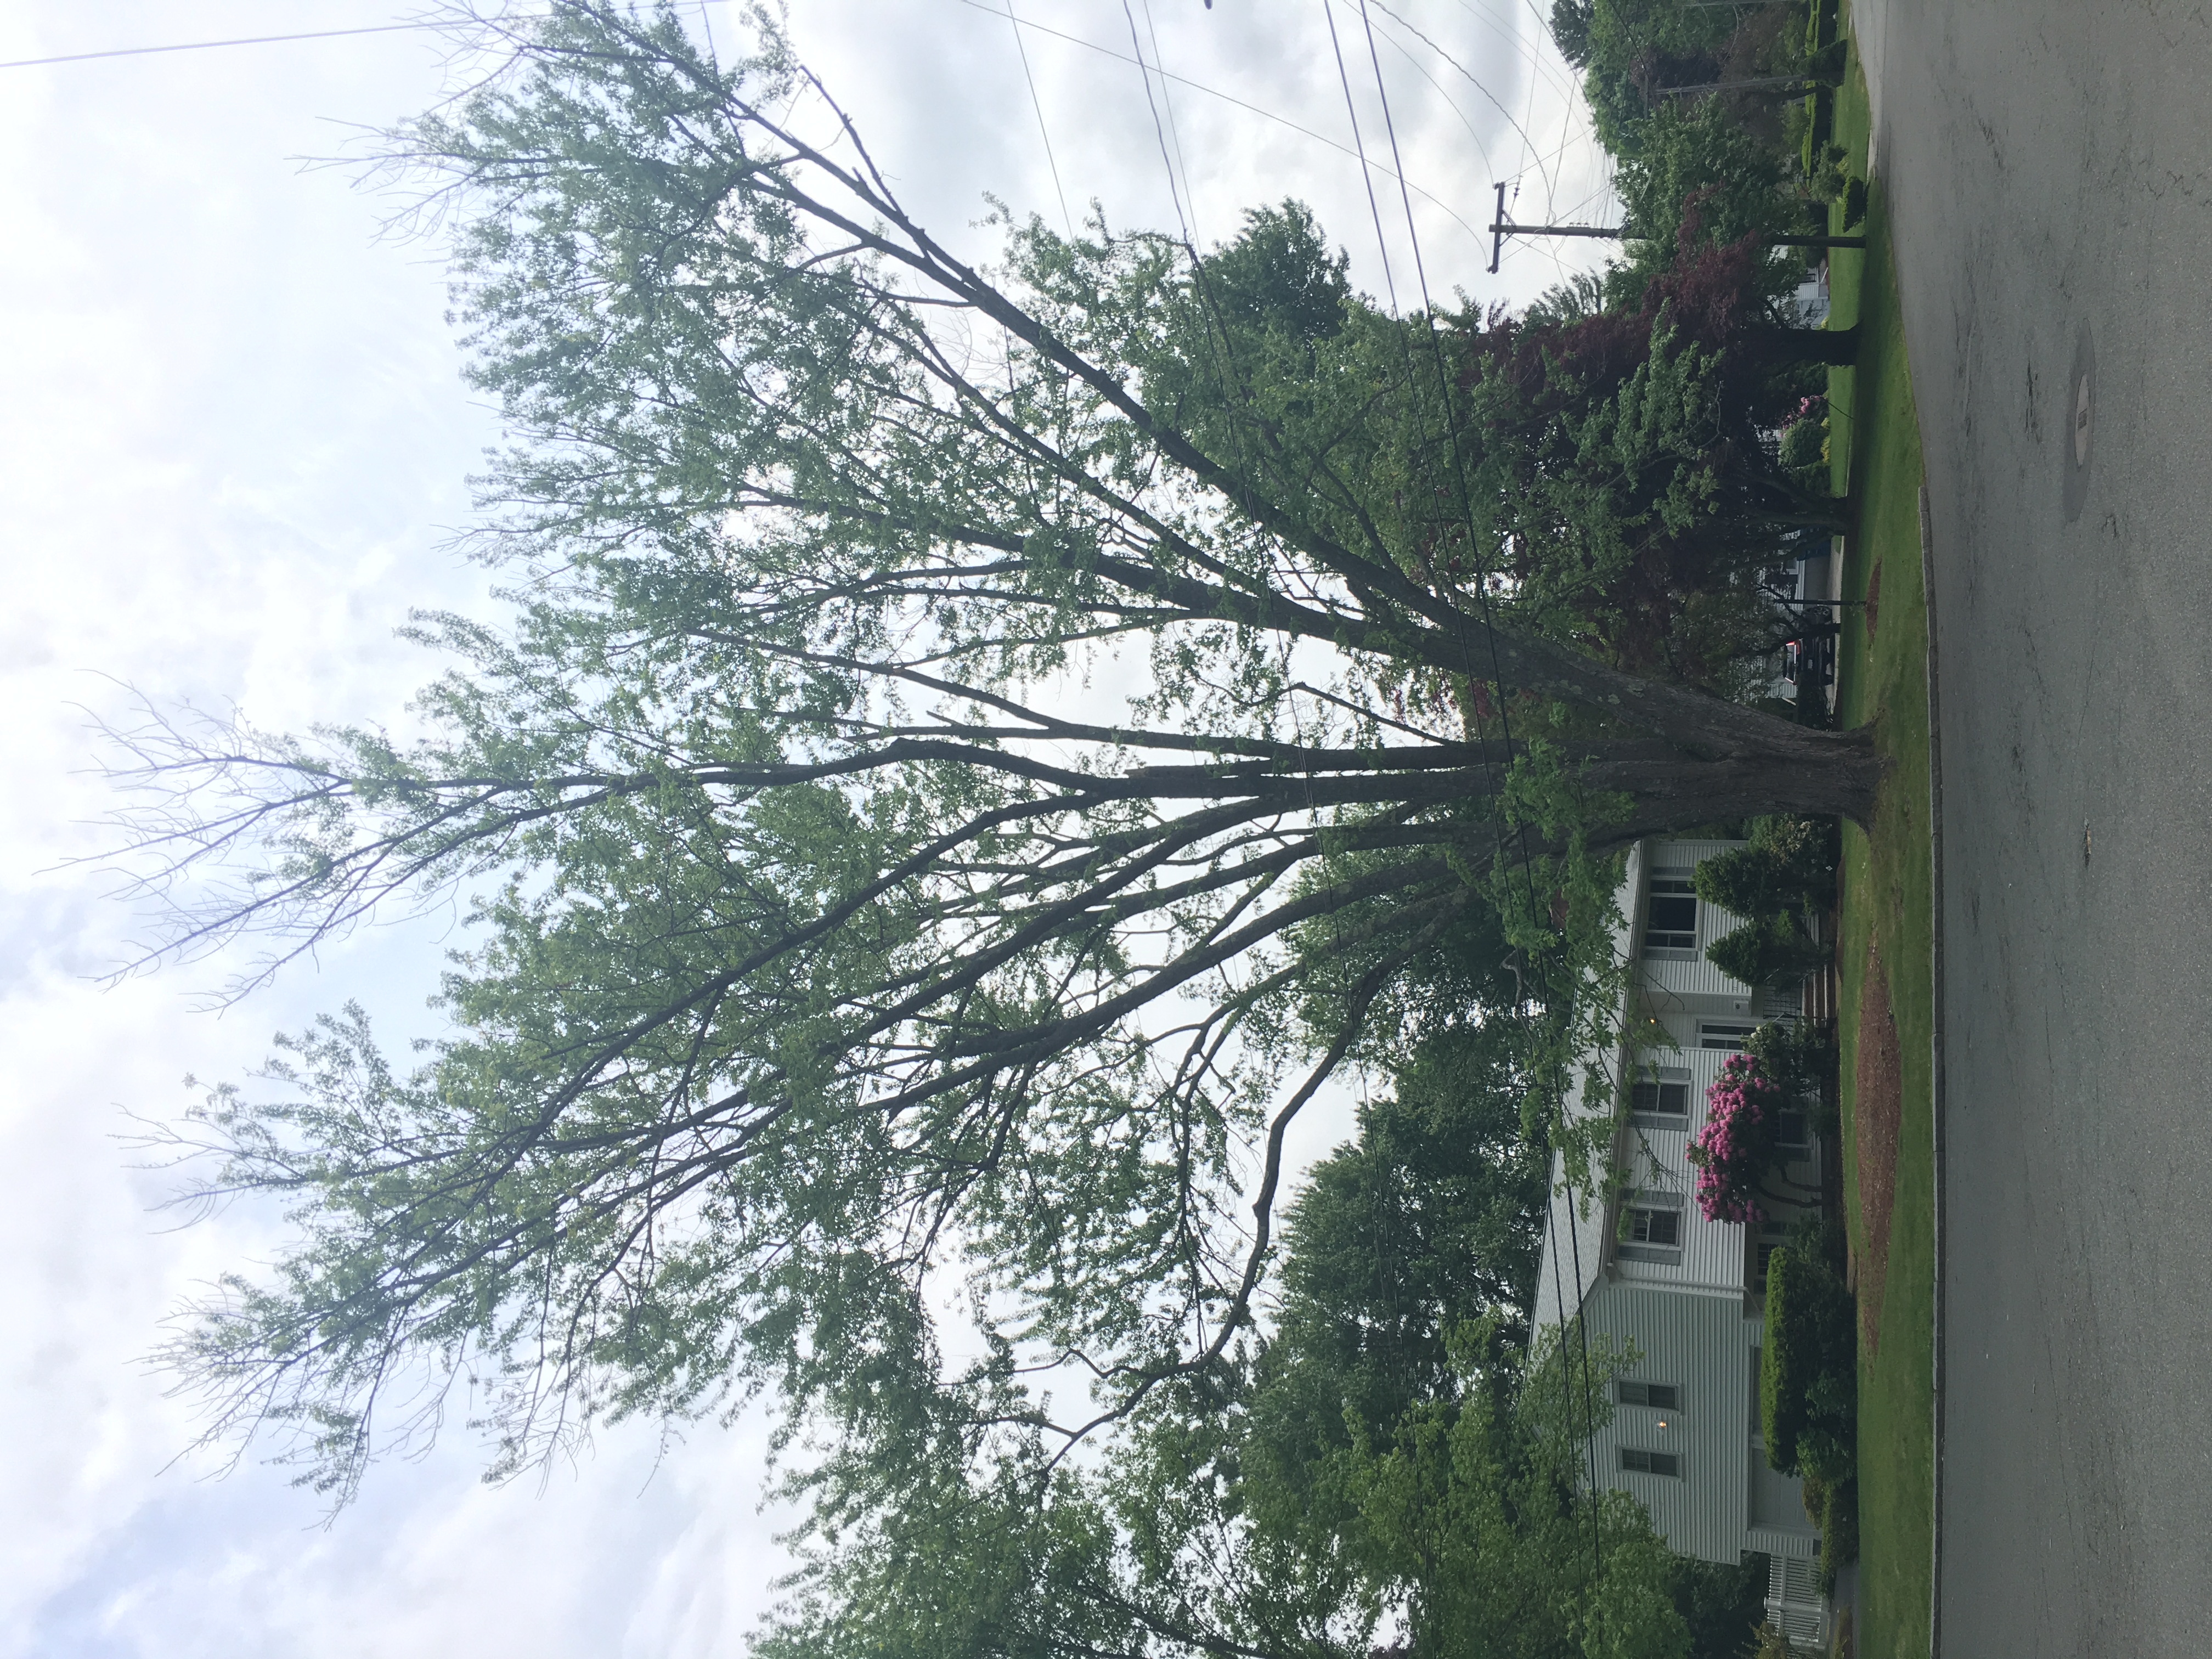
\includegraphics[width=\textwidth,keepaspectratio=true,angle=-90]{possible-example-2} % Possible (silver maple, codom weak attach, reaction wood)
    \caption{Possible}   
  \end{subfigure}
  \begin{subfigure}[t]{.325\linewidth}\centering
    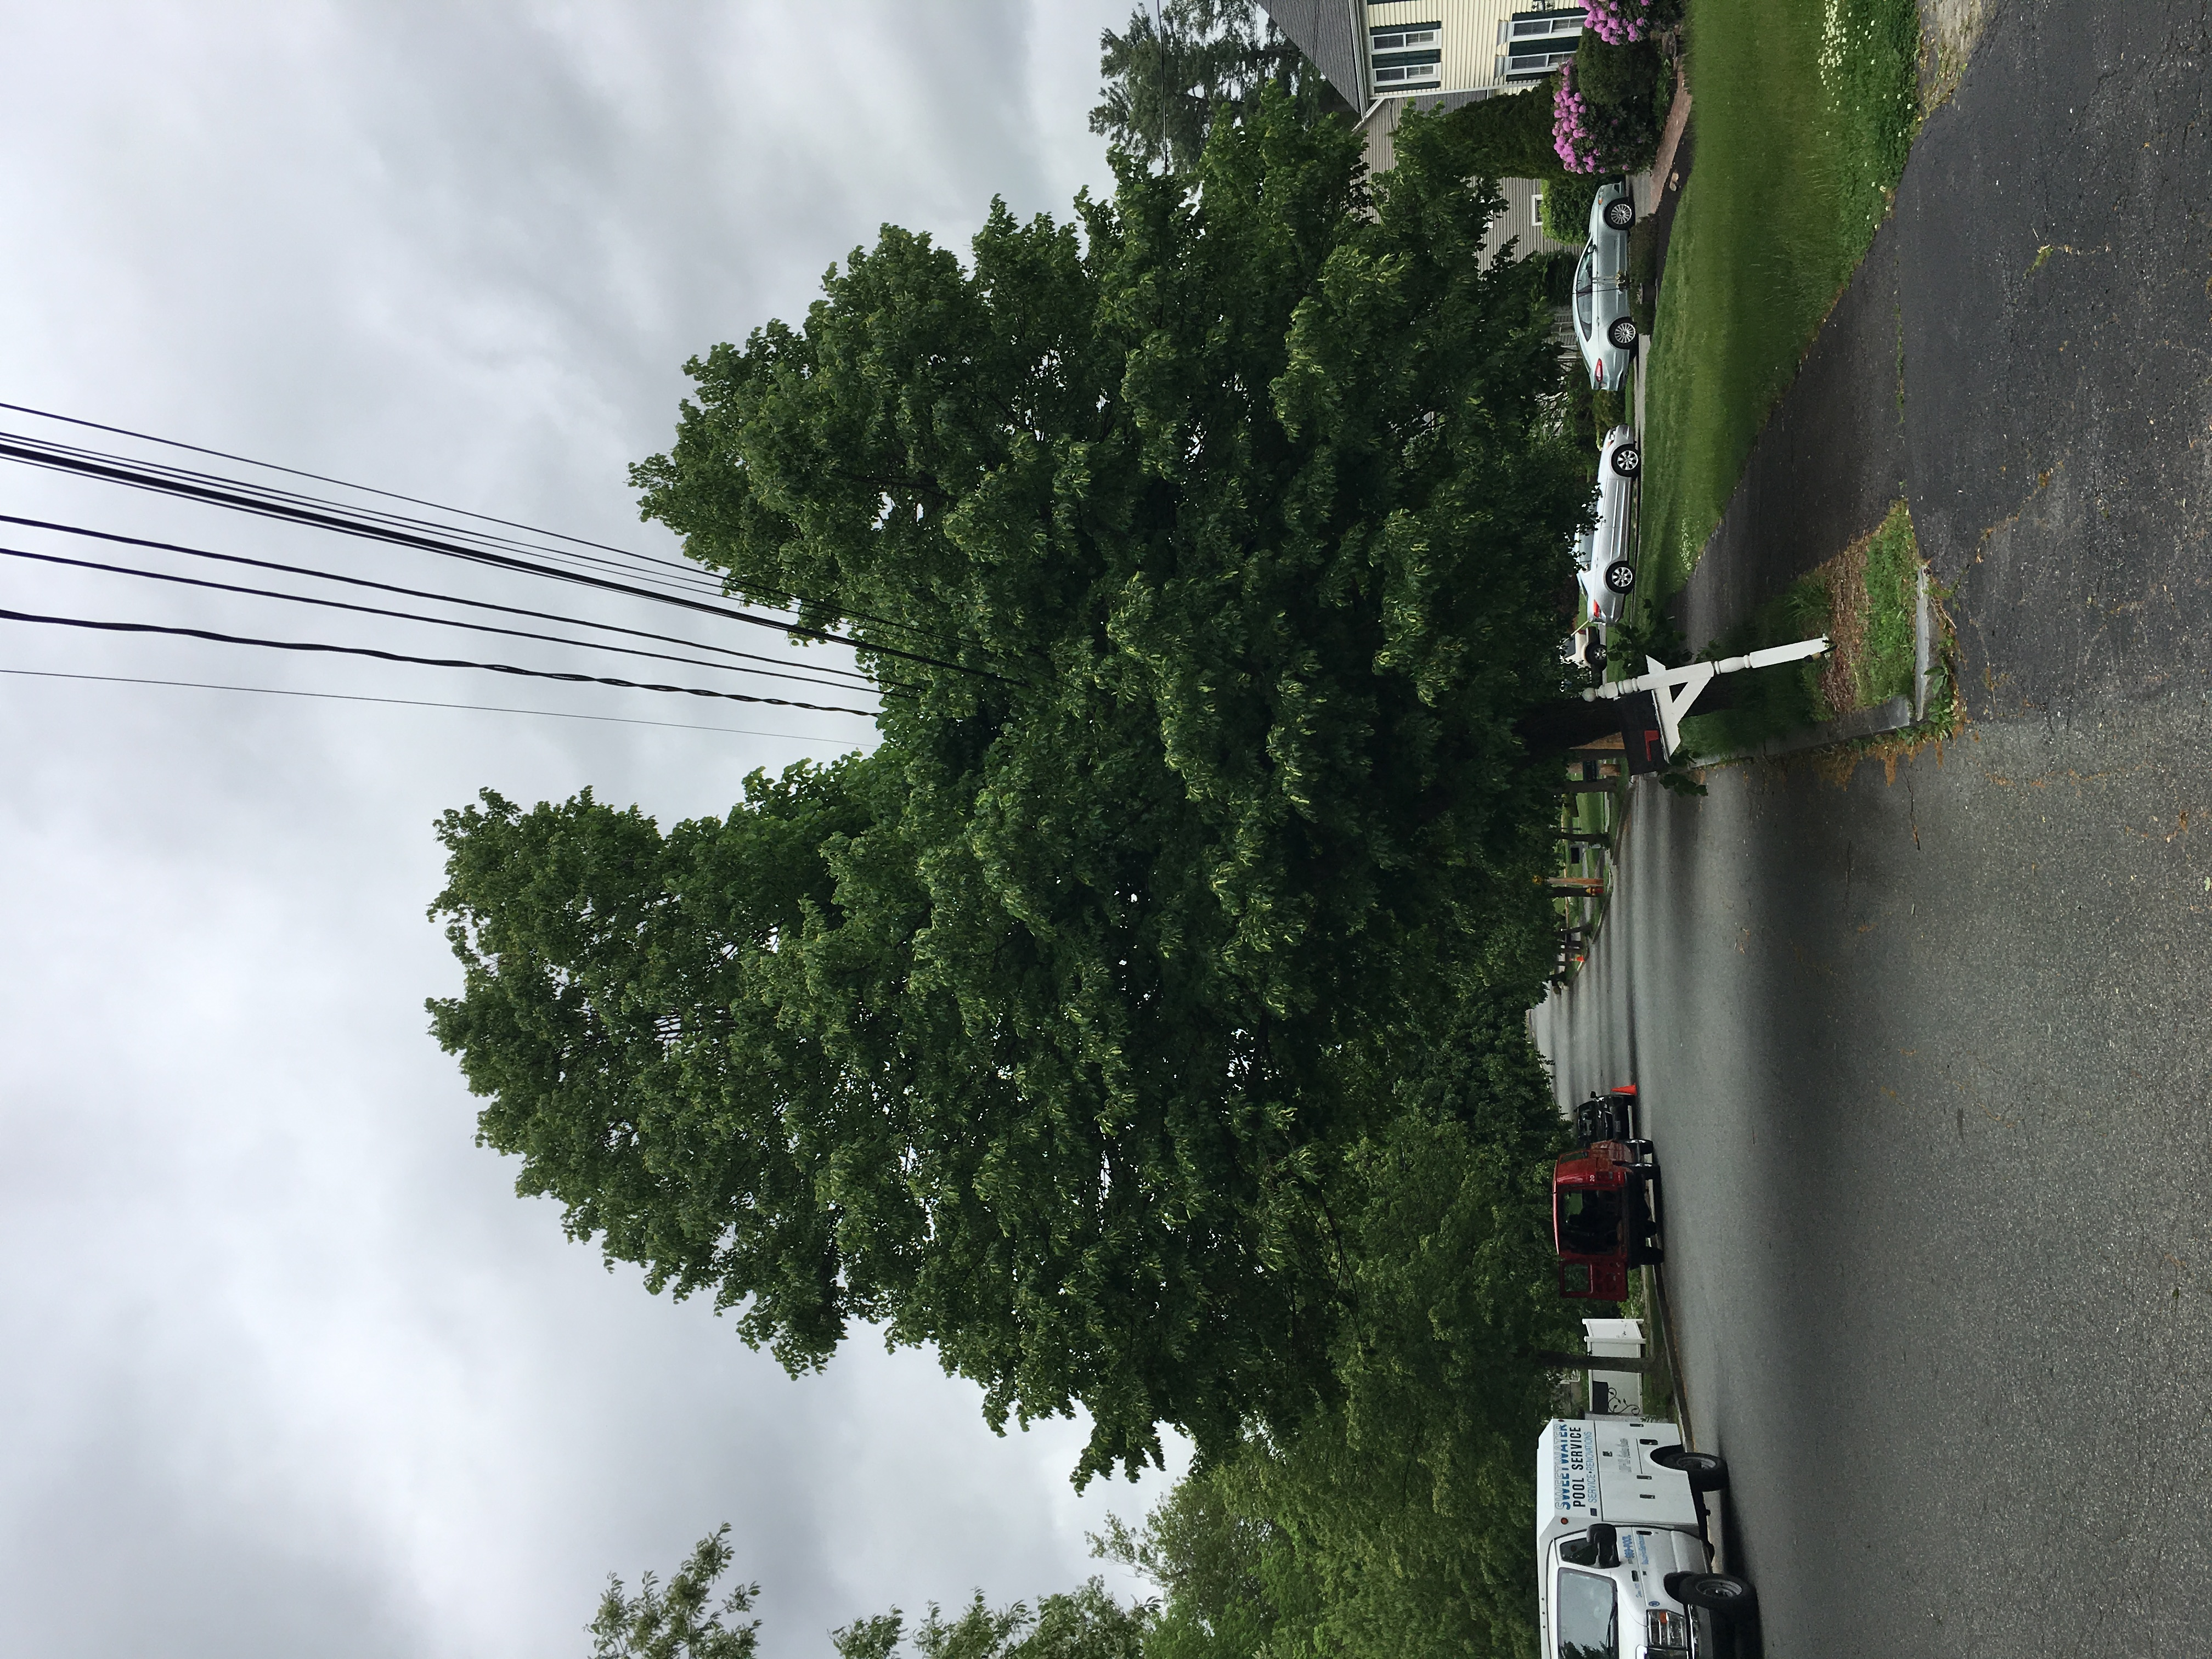
\includegraphics[width=\textwidth,keepaspectratio=true,angle=-90]{improbable-example-1} %Improbable_3_london plane

    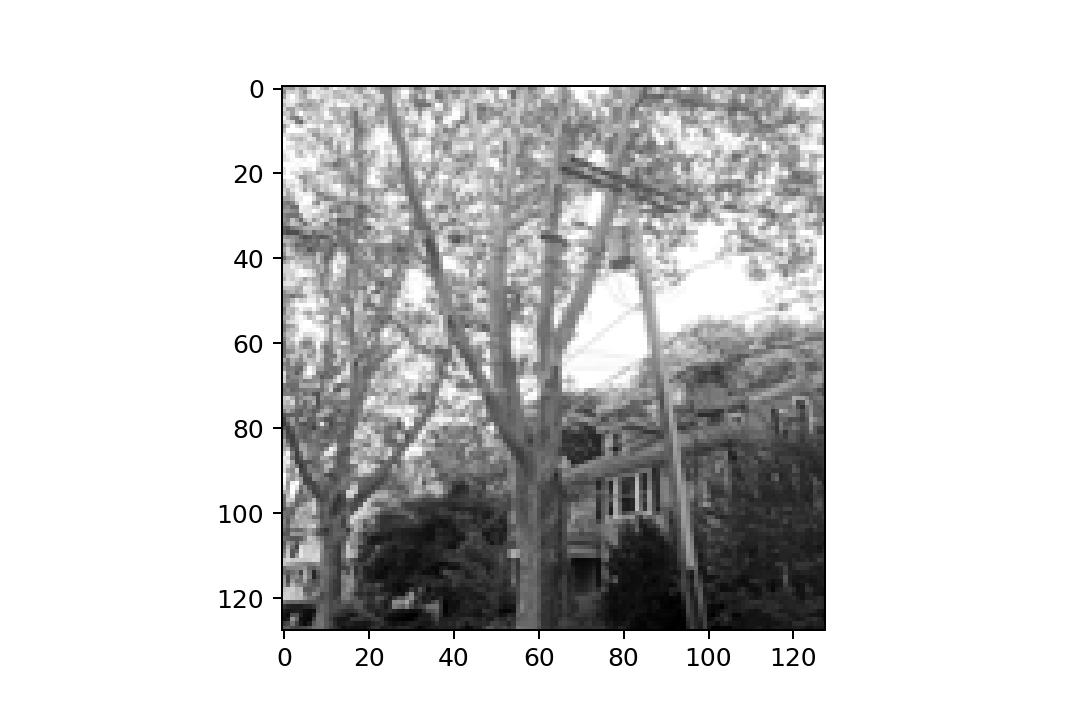
\includegraphics[width=\textwidth,keepaspectratio=true,angle=-90]{improbable-example-2}
    \caption{Improbable}
  \end{subfigure}
  \caption{Examples of training images in each of the three tree risk categories considered in this study.  Trees in  
     column (a) were categorized as \textit{Improbable} due to their lack of structural defects as well as good
    physiological health. Trees in the center column were categorized as \textit{Possible} due to weak branch unions and crown
    dieback. Trees in column (c)  were categorized as \textit{Probable} because they were dead. Leaves in the bottom
    image in the left-hand column are from vines attached to the dead tree.}
  \label{fig:raw_images}
\end{figure}

\begin{table}[h!]\small
    \centering
    \begin{tabular}{l r}\toprule
    \bf Category     & \bf Number of images  \\ \midrule
    \textit{Probable} & 56 \\
      \textit{Possible} & 80 \\
      \textit{Improbable} & 322\\\midrule
    Total & 505 \\\bottomrule
    \end{tabular}
    \caption{Category distribution  in the set of raw input images}
    \label{tab:classdist}
\end{table}


\subsection{Classification scenarios}
In order to investigate the efficacy of an AI classifier to distinguish the failure-likelihood categories, we defined four classification scenarios in \autoref{tab:scenarios} for our experiments. 
Each scenario represents a unique grouping of each of the three categories, with a minimum of two derived classes in each case.
\begin{table}[h!]
    \centering
    \begin{tabular}{l l c}\toprule
    \bf Scenario            & \bf Description  & \bf No.\ classes\\\midrule
    Pr\_Im          & \{\textit{Probable}, \textit{Improbable}\}           & 2 \\
    PrPo\_Im        & \{\textit{Probable} + \textit{Possible}, \textit{Improbable}\}  & 2 \\
    Pr\_PoIm        & \{\textit{Probable}, \textit{Possible} + \textit{Improbable}\}  & 2 \\
    Pr\_Po\_Im     &  \{\textit{Probable}, \textit{Possible}, \textit{Improbable}\} & 3 \\
    \bottomrule
    \end{tabular}
    \caption{Classification scenarios}
    \label{tab:scenarios}
\end{table}

Scenario Pr\_Im considered only the highest and lowest likelihood of failure categories used in the study to clearly distinguish between categories. Since previous research has suggested that professionals more often disagree when distinguishing between possible and probable likelihood of failure \cite{koeser2020can}, in scenario PrPo\_Im, we pooled trees in the \textit{Probable} and \textit{Possible} categories and compared them to trees in the \textit{Improbable} category. In scenario Pr\_PoIm, we pooled trees in the \textit{Possible} and \textit{Improbable} categories and compared them to trees in the \textit{Probable} category. In practice, this scenario is less likely because arborists typically distinguish trees with an \textit{Improbable} likelihood of failure as those with minimal or no structural defects. It requires additional judgment to distinguish trees with probable or possible likelihood of failure because an arborist must assess the severity of structural defects, the presence of response growth, and the expected loads \cite{smiley2017best}. Scenario Pr\_Po\_Im considered each likelihood of failure category separately, as an arborist would do in practice. 

\subsection{Image pre-processing and augmentation}
Data augmentation refers to the variety of methods that are employed for synthetically generating more samples in a training dataset in order to improve model performance \cite{wong2016understanding}.
Augmentation is desired, particularly in situations where the number of original observations is small, and the effectiveness of various relevant techniques in this domain has been amply demonstrated \cite{shorten2019survey}.

In order to achieve robustness in our model, and given the relatively small number of training images, we randomly cropped each image on either axis to 3024 $\times$ 3024 pixels, generating five instances for each one. Thus, we increased the size of our training set from 505 to 2525 images. Further, we performed horizontal flipping with a 50\% probability on each of the generated images. For efficiency, we converted the images to grayscale and scaled the pixel values from 0 to 1. Finally, we downsampled the images to the following resolutions (pixels): $64 \times 64$, $128 \times 128$ and $224 \times 224$, creating a training set for each case. 
Random sets of images from each class across each of the four classification scenarios are shown in \autoref{fig:processed_images}.

\begin{figure}[h!]
  \begin{subfigure}[b]{.24\linewidth}
    \centering
    \textit{\footnotesize Probable}
    
    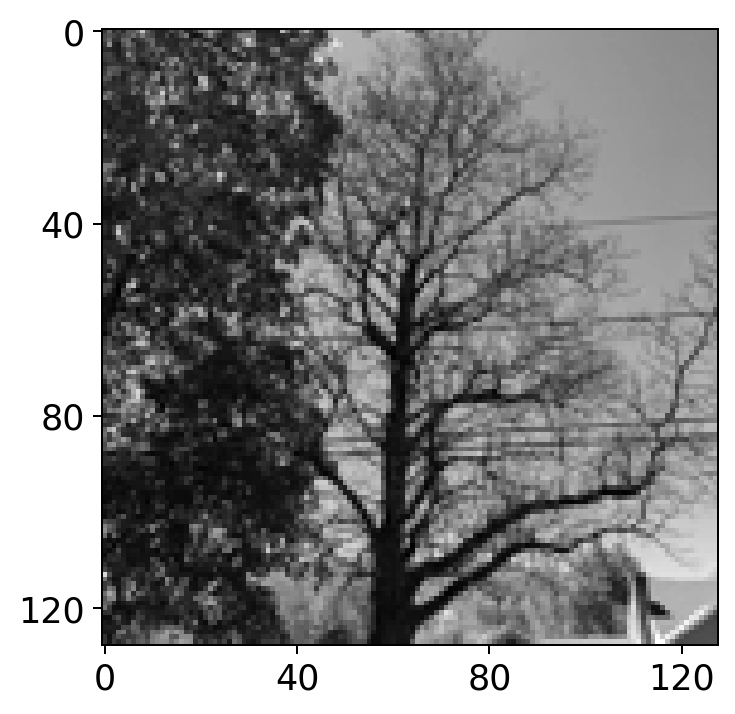
\includegraphics[width=\textwidth]{processed-probable-example-1}
    
    \textit{\footnotesize Improbable}
    
    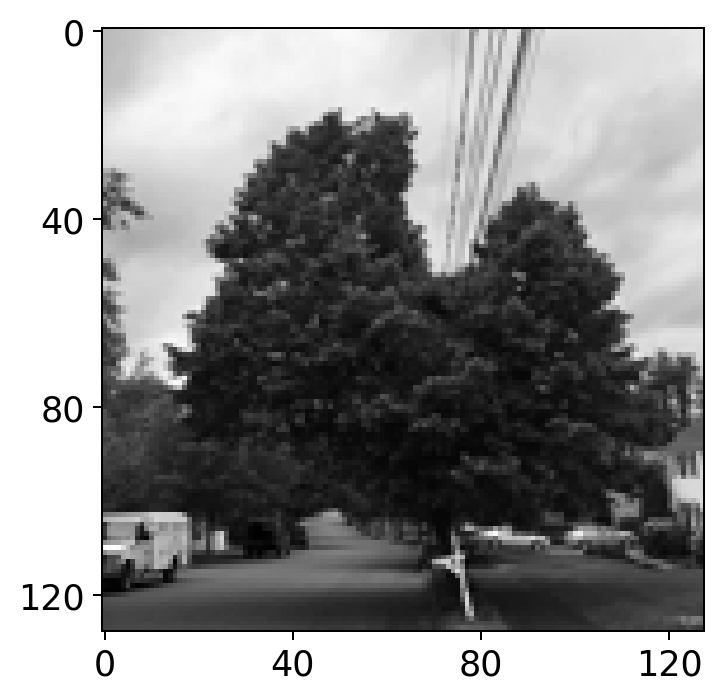
\includegraphics[width=\textwidth]{processed-improbable-example-1}
    \caption{Scenario Pr\_Im}
    \label{pr_im_64}
  \end{subfigure}%
  \begin{subfigure}[b]{.24\linewidth}
    \centering
    \textit{\footnotesize Probable/Possible}
    
    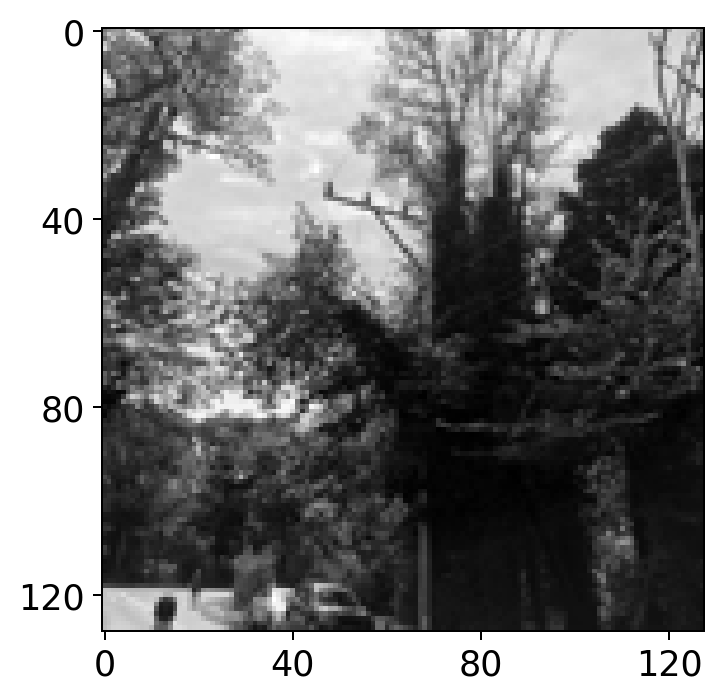
\includegraphics[width=\textwidth]{processed-probable-example-2-flipped}

    \textit{\footnotesize Improbable}
    
    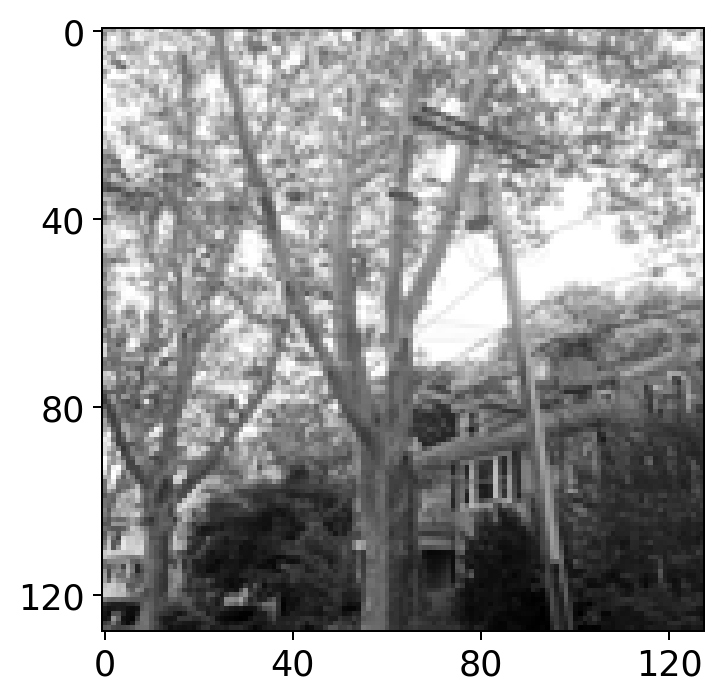
\includegraphics[width=\textwidth]{processed-improbable-example-2}
    \caption{Scenario  PrPo\_Im}
    \label{prpo_im_64}
  \end{subfigure}%  
  \begin{subfigure}[b]{.24\linewidth}
    \centering
    \textit{\footnotesize Probable}
    
    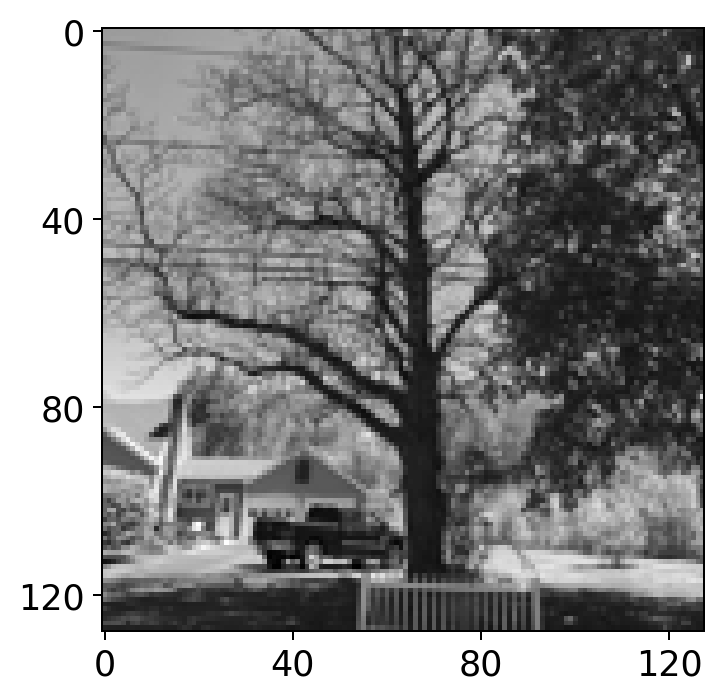
\includegraphics[width=\textwidth]{processed-probable-example-1-flipped}

    \textit{\footnotesize Possible/Improbable}
    
    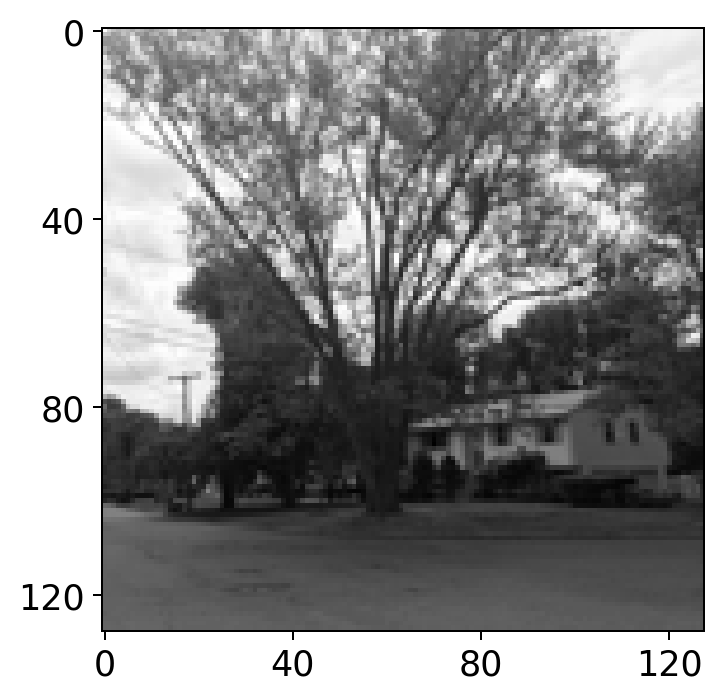
\includegraphics[width=\textwidth]{processed-possible-example-2-flipped}
    \caption{Scenario Pr\_PoIm}
    \label{pr_poim_64}
  \end{subfigure}%  
  \begin{subfigure}[b]{.24\linewidth}
    \centering
    % 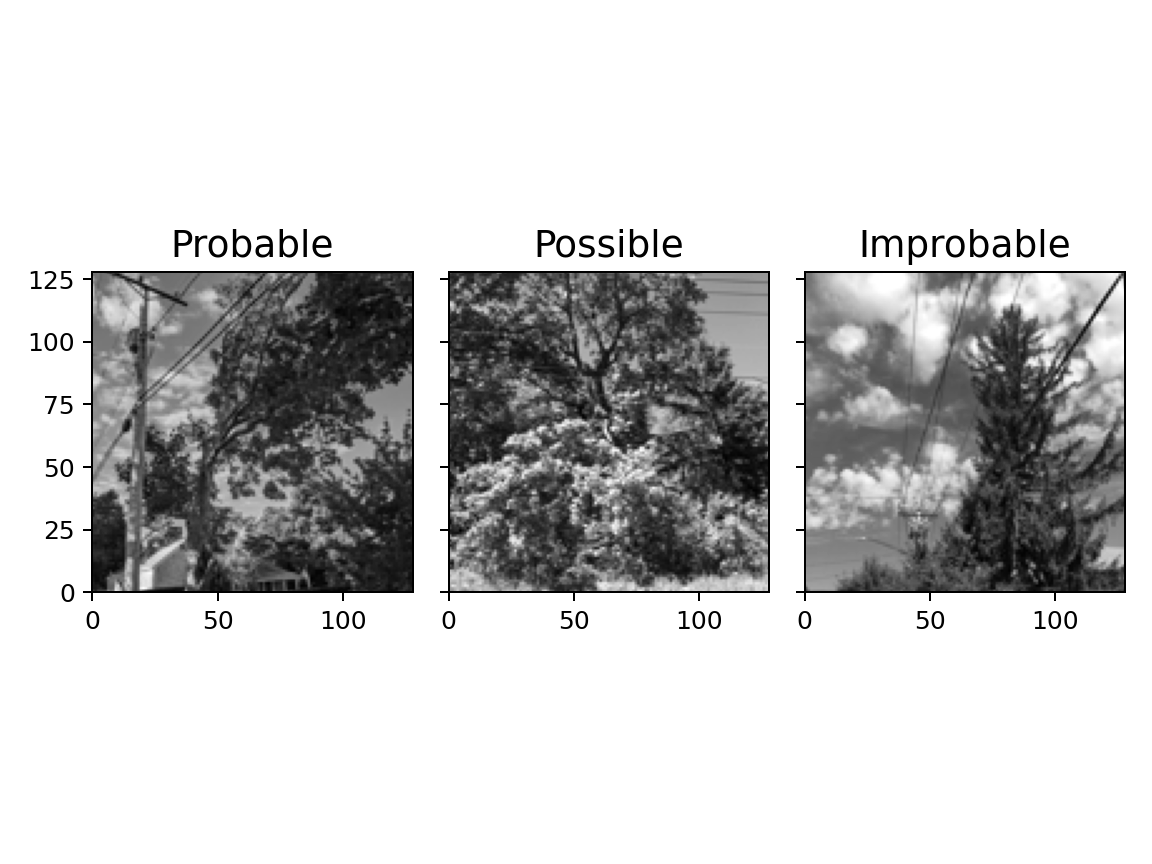
\includegraphics[width=.8\linewidth, trim={0 3cm 0 3cm}, clip]{processed_input_images_Pr_Po_Im_128_px}
    \textit{\footnotesize Probable}
    
    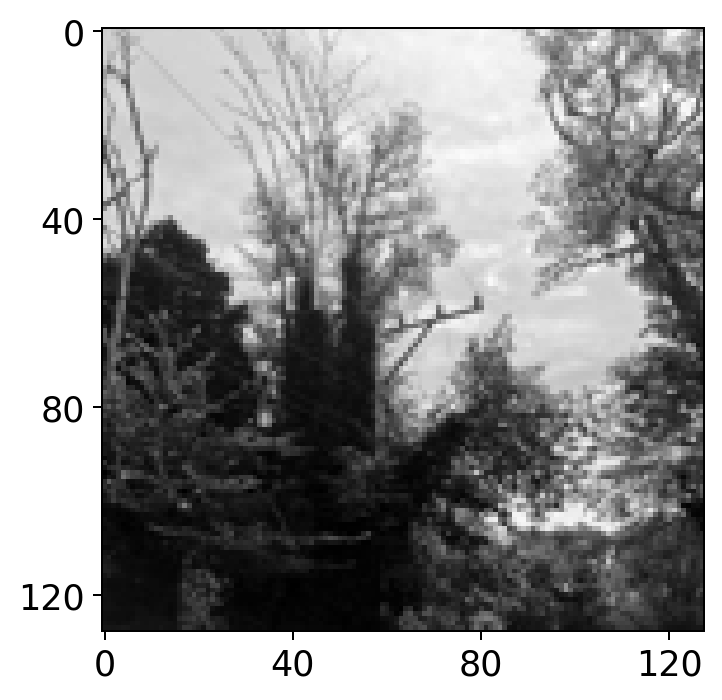
\includegraphics[width=\textwidth]{processed-probable-example-2}

    \textit{\footnotesize Possible}
    
    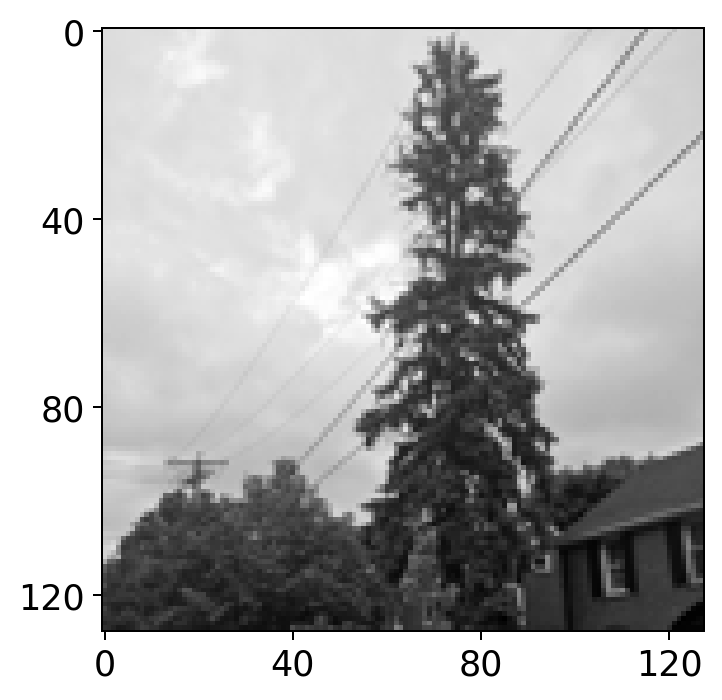
\includegraphics[width=\textwidth]{processed-possible-example-1}
    
    \textit{\footnotesize Improbable}
    
    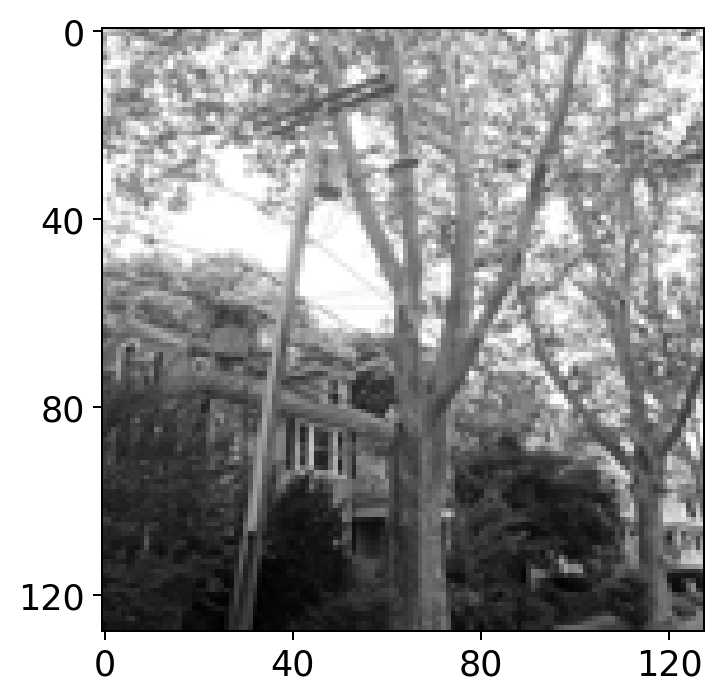
\includegraphics[width=\textwidth]{processed-improbable-example-2-flipped}
    \caption{Scenario Pr\_Po\_Im}
    \label{pr_po_im_64}
  \end{subfigure}%
  
  \caption{Selected processed training images under each classification scenario.
    The images shown are processed versions of those shown in \autoref{fig:raw_images}.
    All were randomly cropped along the vertical axis and 50\% were horizontally flipped (including some in this figure).
  }
  \label{fig:processed_images}
\end{figure}

\subsection{Convolutional neural network}
% We can apply cut-out (occluding portions of the image) for improved performance \cite{devries2017improved}. Also, it has been shown that training with lower resolution improves performance on higher resolution test images \cite{touvron2019fixing}.
We employ a convolutional neural network (CNN) as the AI framework for tree risk failure likelihood prediction.  Like
other neural networks, the CNN is an arrangement of neurons within layers, each neuron performing an operation that maps
from a pixel in an input image to the final output.  The input into each neuron is a weighted sum from the previous
layer, while the output from each neuron is modulated by an activation function.  The activation function in the final
layer of an CNN is typically the softmax function, which gives the class probabilities of a given input image.  A class
is assigned to the image based on the one with the corresponding maximum probability.

Unlike other neural networks, however, the CNN performs fundamental pixel-mapping operations in its convolutional
layers. Each convolutional layer is defined by a stack of feature maps, which result from a dot product of a filter and
correspondinlgy-sized local receptive fields from the input image or preceding layer.  The numeric values of the filters
correspond to weights whose optimal values are learned during the training of the CNN.  The size of the filter in each
convolutional layer is given by the \textit{kernel size}.

In this paper, we employ a relatively simple CNN architecture, historically inspired by AlexNet \cite{krizhevsky2012imageneta}.
The structure of the CNN is shown in \autoref{fig:cnn} (generated using an automated  framework \cite{bauerle2021net2vis}).
After the input layer (a matrix of pixels from the input image), we use a 64-filter convolutional layer.
The output is downsampled using a pooling layer that returns the maximum output from a $2\times 2$ subsample from the previous layer.
Next, we stack two successive convolutional layers each with a depth of 128 filters.
We follow these with a maximum-pooling layer and then two further 256-filter convolutional layers.
A final maximum-pooling layer is used before we ``flatten'' all outputs into a one-dimensional (fully-connected) array of neurons. 
After flattening the outputs, we use a dense layer to reduce the number of outputs a specified number of units.
Batch normalization \cite{ioffe2015batch} is employed after the first dense layer to improve training efficiency.
A second dense layer is used prior to the output layer, with the number of outputs corresponding to the number of classes in the dataset.
A regularization technique known as ''dropout'' is used after each dense layer.
In each dropout layer, a proportion of the neurons are randomly zeroed during training in order to improve the robustness of the model.
\begin{figure}
    \centering
    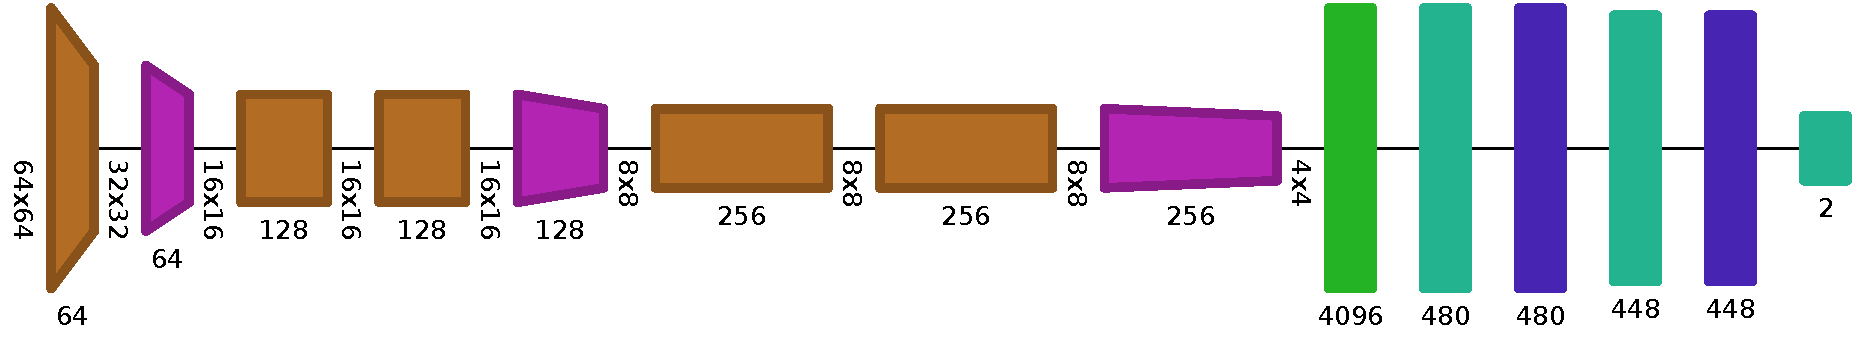
\includegraphics[width=.9\textwidth]{net2vis/graph.pdf}
    
    \bigskip
    
    
\includegraphics[width=.5\textwidth, trim={4cm 0 0 0}, clip]{figures/net2vis-name-labels/legend}
    \caption{Diagram of convolutional neural network structure (excluding the input layer). Hyperparameters that are
      optimized include the number of units in the penultimate dense layers. Here, 480 and 448 units are used, respectively.}
    \label{fig:cnn}
\end{figure}

The various hyperparameters in the model are summarized in \autoref{tab:hyp}.
\begin{table}[]\small
\rowcolors{1}{white}{gray!35}
    \centering
    \begin{tabular}{l c c c c c c c}\toprule
    \bf Layer & \bf Layer \# & \bf No.\ Filters & \bf Kernel Size & \bf Strides &
    \bf Activation &   \bf Rate & \bf No.\ Units  \\\midrule
    Convolutional  & 1         & 64                & $k$   & 2           & ReLU && \\
    Max. Pooling   & 1         &                   & 2               &&&             &      \\
    Convolutional  & 2         & 128               & 3   & 1           & ReLU && \\
    Convolutional  & 3         & 128               & 3   & 1           & ReLU && \\
    Max. Pooling   & 2         &                   & 2               &&&             &      \\    
    Convolutional  & 4         & 256               & 3   & 1           & ReLU && \\
    Convolutional  & 5         & 256               & 3   & 1           & ReLU && \\
    Max. Pooling   & 3         &                   & 2               &             &&&      \\\midrule
    Flatten & & & & &&& \\\midrule
%     &  &   &  & & &
%     \bf Rate & \bf No.\ Units  \\\midrule
    Dense           & 1  & & &  &  $a_1$ & & $u_1$ \\
    Dropout         & 1  & & &  && $r_1$ &   \\
    Dense           & 2  & & &  &  $a_2$ & & $u_2$  \\
    Dropout         & 2  & & &  && $r_2$ &  \\ \bottomrule
    \end{tabular}
    \caption{Summary of the convolutional neural network hyperparameters. 
    Those represented by a symbol are optimized using a guided search.}
    \label{tab:hyp}
\end{table}

\subsection{Hyperparameter optimization}
We optimized eight of the CNN hyperparameters using Hyperband \cite{li2018hyperband}, an efficient guided grid-search algorithm.
Twelve searches were performed for each classification scenario and image resolution combination.
Each search was conducted using 90 trials of unique hyperparameter combinations. The specified range of each parameter along with the search results are shown in \autoref{tab:opt-hyp}. For the kernel size in the first convolutional layer, we allowed for a choice between a $5\times 5$ and a $7\times 7$ kernel. The activation function in both dense layers was specified as a choice between the rectified linear unit (ReLU) function and the hyperbolic tangent ($\tanh$). The ReLU was introduced to address the so-called ``vanishing gradient'' problem and has been shown to improve performance in CNNs \cite{glorot2011deep}. Nevertheless, the $\tanh$ function remains a viable option, as well. The dropout rates were allowed to range from 0 to 5 in steps of 0.05, while the number of neurons or units in each dense layer varied from 32 to 512 in steps of 32. Finally, we uniformly sampled learning rates for the optimizer in the $\log_{10}$ space of $[10^{-4}, 10^{-2}]$.

\begin{table}[ht!]\small
%\rowcolors{7}{white}{gray!35}
    \centering
    \sisetup{round-mode=places,
        round-precision=2,
        scientific-notation=fixed,
        exponent-product = \cdot,
        table-omit-exponent,
        fixed-exponent=-4
        }
% Please add the following required packages to your document preamble:
% \usepackage{booktabs}
% \usepackage{multirow}
\begin{tabular}{@{}lllccc@{}}
\toprule
\multirow{2}{*}{\textbf{Scenario}} & \multirow{2}{*}{\textbf{Hyperparameter}} & \multirow{2}{*}{\textbf{Range}} & \multicolumn{3}{c}{\textbf{Resolution}} \\ \cmidrule(l){4-6} 
                          &                              &                           & \textbf{64}             & \textbf{128}            & \textbf{224}            \\ \midrule
\multirow{8}{*}{Pr\_Im}    & 1st conv. kernel size, $k$   & $\{5, 7\}$                & 7                       & 7                       & 7                       \\
                          & 1st dense activation, $a_1$  & \{ReLU, $\tanh$\}         & ReLU                    & ReLU                    & ReLU                    \\
                          & 2nd dense activation, $a_2$  & \{ReLU, $\tanh$\}         & ReLU                    & ReLU                    & ReLU                    \\
                          & 1st dropout rate, $r_1$      & $\{0, .05, \ldots, 5\}$   & 0.1                     & 0.1                     & 0.1                     \\
                          & 2nd dropout rate, $r_2$      & $\{0, .05, \ldots, 5\}$   & 0.3                     & 0.3                     & 0.3                     \\
                          & 1st dense layer units, $u_1$ & $\{32, 64, \ldots, 512\}$ & 480                     & 480                     & 480                     \\
                          & 2nd dense layer units, $u_2$ & $\{32, 64, \ldots, 512\}$ & 448                     & 448                     & 448                     \\
                          & learning rate, $\lambda$     & $[10^{-4}, 10^{-2}]$      & \num{0.000102956216062} & \num{0.000102956216062} & \num{0.000102956216062} \\\midrule
\multirow{8}{*}{PrPo\_Im}  & 1st conv. kernel size, $k$   & $\{5, 7\}$                & 7                       & 5                       & 7                       \\
                          & 1st dense activation, $a_1$  & \{ReLU, $\tanh$\}         & ReLU                    & tanh                    & ReLU                    \\
                          & 2nd dense activation, $a_2$  & \{ReLU, $\tanh$\}         & ReLU                    & ReLU                    & ReLU                    \\
                          & 1st dropout rate, $r_1$      & $\{0, .05, \ldots, 5\}$   & 0.1                     & 0.25                    & 0.1                     \\
                          & 2nd dropout rate, $r_2$      & $\{0, .05, \ldots, 5\}$   & 0.3                     & 0.35                    & 0.3                     \\
                          & 1st dense layer units, $u_1$ & $\{32, 64, \ldots, 512\}$ & 480                     & 384                     & 480                     \\
                          & 2nd dense layer units, $u_2$ & $\{32, 64, \ldots, 512\}$ & 448                     & 256                     & 448                     \\
                          & learning rate, $\lambda$     & $[10^{-4}, 10^{-2}]$      & \num{0.000102956216062} & \num{0.000109137476524} & \num{0.000102956216062} \\\midrule
\multirow{8}{*}{Pr\_PoIm}  & 1st conv. kernel size, $k$   & $\{5, 7\}$                & 7                       & 7                       & 7                       \\
                          & 1st dense activation, $a_1$  & \{ReLU, $\tanh$\}         & ReLU                    & ReLU                    & ReLU                    \\
                          & 2nd dense activation, $a_2$  & \{ReLU, $\tanh$\}         & tanh                    & ReLU                    & tanh                    \\
                          & 1st dropout rate, $r_1$      & $\{0, .05, \ldots, 5\}$   & 0.25                    & 0.1                     & 0.2                     \\
                          & 2nd dropout rate, $r_2$      & $\{0, .05, \ldots, 5\}$   & 0.3                     & 0.3                     & 0.15                    \\
                          & 1st dense layer units, $u_1$ & $\{32, 64, \ldots, 512\}$ & 128                     & 480                     & 416                     \\
                          & 2nd dense layer units, $u_2$ & $\{32, 64, \ldots, 512\}$ & 320                     & 448                     & 416                     \\
                          & learning rate, $\lambda$     & $[10^{-4}, 10^{-2}]$      & \num{0.000175822328104} & \num{0.000102956216062} & \num{0.000114656409879} \\\midrule
\multirow{8}{*}{Pr\_Po\_Im} & 1st conv. kernel size, $k$   & $\{5, 7\}$                & 7                       & 5                       & 7                       \\
                          & 1st dense activation, $a_1$  & \{ReLU, $\tanh$\}         & ReLU                    & tanh                    & ReLU                    \\
                          & 2nd dense activation, $a_2$  & \{ReLU, $\tanh$\}         & tanh                    & ReLU                    & ReLU                    \\
                          & 1st dropout rate, $r_1$      & $\{0, .05, \ldots, 5\}$   & 0.25                    & 0.25                    & 0.1                     \\
                          & 2nd dropout rate, $r_2$      & $\{0, .05, \ldots, 5\}$   & 0.3                     & 0.35                    & 0.3                     \\
                          & 1st dense layer units, $u_1$ & $\{32, 64, \ldots, 512\}$ & 128                     & 384                     & 480                     \\
                          & 2nd dense layer units, $u_2$ & $\{32, 64, \ldots, 512\}$ & 320                     & 256                     & 448                     \\
                          & learning rate, $\lambda$     & $[10^{-4}, 10^{-2}]$      & \num{0.000175822328104} & \num{0.000109137476524} & \num{0.000102956216062} \\ \bottomrule
\end{tabular}
\caption{Optimal hyperparameters found using the Hyperband search algorithm for 12 classification scenario and input image resolution combinations.}
    \label{tab:opt-hyp}
\end{table}

\subsection{Model training and assessment}
In this subsection, we provide an overview of the learning procedure for the convolutional neural network.
As a reference, all the symbols used here are summarized in \autoref{tab:symbols}

\begin{table}[h!]
    \centering
    \begin{tabular}{l l c}\toprule
    \bf Symbol            & \bf Definition  \\\midrule
      $c$          & \ Index of given class\\
      $f(s_c)$        & \ Softmax activation function \\
      $F_{1c}$ & \ Class-specific  $F_1$ score \\      
      $F_1^m$ & \ Macro-average $F_1$ score \\
      $i$     &  \ Index of given image observation \\           
      $L^{CE}_i$        & \ Categorical cross entropy loss function of a single observation \\
      $\hat{p}_{i,c}$        & \ Predicted probability that the $i$\textsuperscript{th} observation belongs to class $c$ \\      
    $Pr_c$ & \ Class-specific precision \\
      $Pr^m$ & \ Macro-average precision \\
      $Re_c$ & \ Class-specific recall \\
      $Re^m$ & \ Macro-average recall \\
          $s_c$        & \ Class-specific score \\
    $y_i$        & \ Observed (true) class of a given observation \\
      $\hat y_i$       & \ Predicted class of a given observation \\
      \bottomrule
    \end{tabular}
    \caption{Summary of symbols related to the training and assessment of the convolutional neural network}
    \label{tab:symbols}
\end{table}
  
The softmax activation function  $f(\cdot)$ in the output layer returns the class prediction probabilities for a given observation $i$. It is defined in terms of the class-specific score $s_c$ as:
\begin{equation}
    f(s_c) = \frac{e^{s_c}}{\sum\limits_{c' \in C} e^{s_{c'}}}
\end{equation}
where $C$ is the set of classes and $c, c'$ are indices for a given class.
Thus for the $i$th observation, the softmax activation returns the predicted probability $\hat{p}_{i,c}$ that the $i$th observation belongs to class $c$.
The CNN is trained using a variant of the stochastic gradient algorithm, Adam \cite{kingma2017adam}.
The goal of the training procedure is to learn the optimal weights and bias terms for the CNN by minimizing a loss function. 
In this case, we use the categorical cross-entropy loss function, which for a single observation can be simply defined as:
\begin{equation}
    L_{i}^{CE} = -  \log( \hat{p}_{i,c}) = - \log(f(s_c^i))
\end{equation}
Training is iteratively performed, with gradient of the loss function computed and averaged over a batch of input images.
Here, we use a batch size of 32.
The learning rate  of the optimization algorithm is an important hyperparameter that affects training performance.
We optimized for this in the hyperparameter search as discussed.
Furthermore, the CNN is trained over multiple passes through the entire training set.
Each such pass is referred to as an epoch.

In real terms, we measured the performance of the trained CNN by how accurately it predicts the classes in a validation set excluded from the training set. For this paper, we used a randomly sampled validation that was 20\% of the size of the input dataset of 2525 images in each training instance.
Thus, we define the accuracy as the overall proportion of correct predictions across all classes.
This metric was computed both for the training and validation sets in each epoch.
In addition to overall accuracy of making correct classifications, we assessed the models trained under these scenarios based on the macro-averages of the precision, recall and $F_1$ score metrics computed over the validation set in each epoch. The precision score $Pr_{c}$ captures the proportion of correct predictions for a certain class relative to all the predictions for that class, and is an important measure of how good a classifier is. The recall $Re_{c}$ captures the ability of a classifier to correctly predict observations for a certain class relative to all the true observations in that class. The $F_{1c}$ metric is given as the class-specific harmonic mean of the precision and recall, and is thus more sensitive than the overall accuracy score. These three metrics are macro-averaged. Thus, each category is given equal weight, ensuring that misclassifications within the smaller classes (\textit{Probable} and \textit{Possible}) are adequately represented in the aggregation. These metrics are formally defined as follows:
\begin{align}
\text{Macro-average precision: }    Pr^m &= \frac{1}{|C|}\sum_{c\in C} \left(  \frac{ \mathrm{TP}_{c} }{\mathrm{TP}_{c} + \mathrm{FP}_c}\right) \\
\text{Macro-average recall: }    Re^m &= \frac{1}{|C|} \sum_{c\in C} \left(  \frac{ \mathrm{TP}_{c} }{\mathrm{TP}_{c} + \mathrm{FN}_c}\right) \\
\text{Macro-average $F_1$ score: }    F_1^m &= \frac{1}{|C|} \sum_{c\in C} \left(  \frac{2  \mathrm{Pr}_{c} \mathrm{Re}_{c}}{\mathrm{Pr}_{c} + \mathrm{Re}_c}\right)
\end{align}
% \begin{align}
% \text{Weighted average precision: }    \mathrm{Pr}^w &= \frac{1}{\sum_{c\in C} n_c} \sum_{c\in C} \left(  \frac{n_c \mathrm{TP}_{c} }{\mathrm{TP}_{c} + \mathrm{FP}_c}\right) \\
% \text{Weighted average recall: }    \mathrm{Re}^w &= \frac{1}{\sum_{c\in C} n_c} \sum_{c\in C} \left(  \frac{n_c \mathrm{TP}_{c} }{\mathrm{TP}_{c} + \mathrm{FN}_c}\right) \\
% \text{Weighted average $F_1$ score: }    F_1^w &= \frac{1}{\sum_{c\in C} n_c} \sum_{c\in C} \left(  \frac{2 n_c \mathrm{Pr}_{c} \mathrm{Re}_{c}}{\mathrm{Pr}_{c} + \mathrm{Re}_c}\right)
% \end{align}
where $c$ is the index of a class in the set $C$ and $|C|$ the number of classes in the dataset. 
The class-specific prediction metrics are given by:
\begin{align}
    \text{True positives for class $c$: } \mathrm{TP}_c &= \sum_{i \in c} I(\hat{y}_i = y_i ) \\
    \text{False positives for class $c$: } \mathrm{FP}_c &= \sum_{i \in c} I(\hat{y}_i \in c | y_i \notin c) \\
    \text{False negatives for class $c$: } \mathrm{FN}_c &= \sum_{i \in c} I(\hat{y}_i \notin c | y_i \in c)
\end{align}
where $\hat y_i$ is the predicted class and $y_i$ the observed (true) class for a given image $i$ in class $c$. The indicator function $I(\cdot)$ returns 1 if the corresponding condition is true, and 0 otherwise.

\section{Results}
We trained the CNN for each of the 4 classification scenarios. In each scenario, we also trained on three image resolution sets (64, 108 and 224). The goal was to determine the best performing resolution, given the tradeoff between performance and computational expenditure. Thus, we generated twelve learning cases. In each case, we performed a 5-fold cross-validation (resulting in a training-validation ratio of 80:20 in each fold).
We trained the CNN over 20 epochs in all the cases. The trajectories of the  loss and accuracy are shown in \autoref{fig:sens-overall} for both the training and validation sets. % Although the 64-pixel case is the slowest to converge in all scenarios, it appears to have a similar performance with respect to the other two resolutions (128px and 224px).

\begin{figure}[ht]
    \centering
    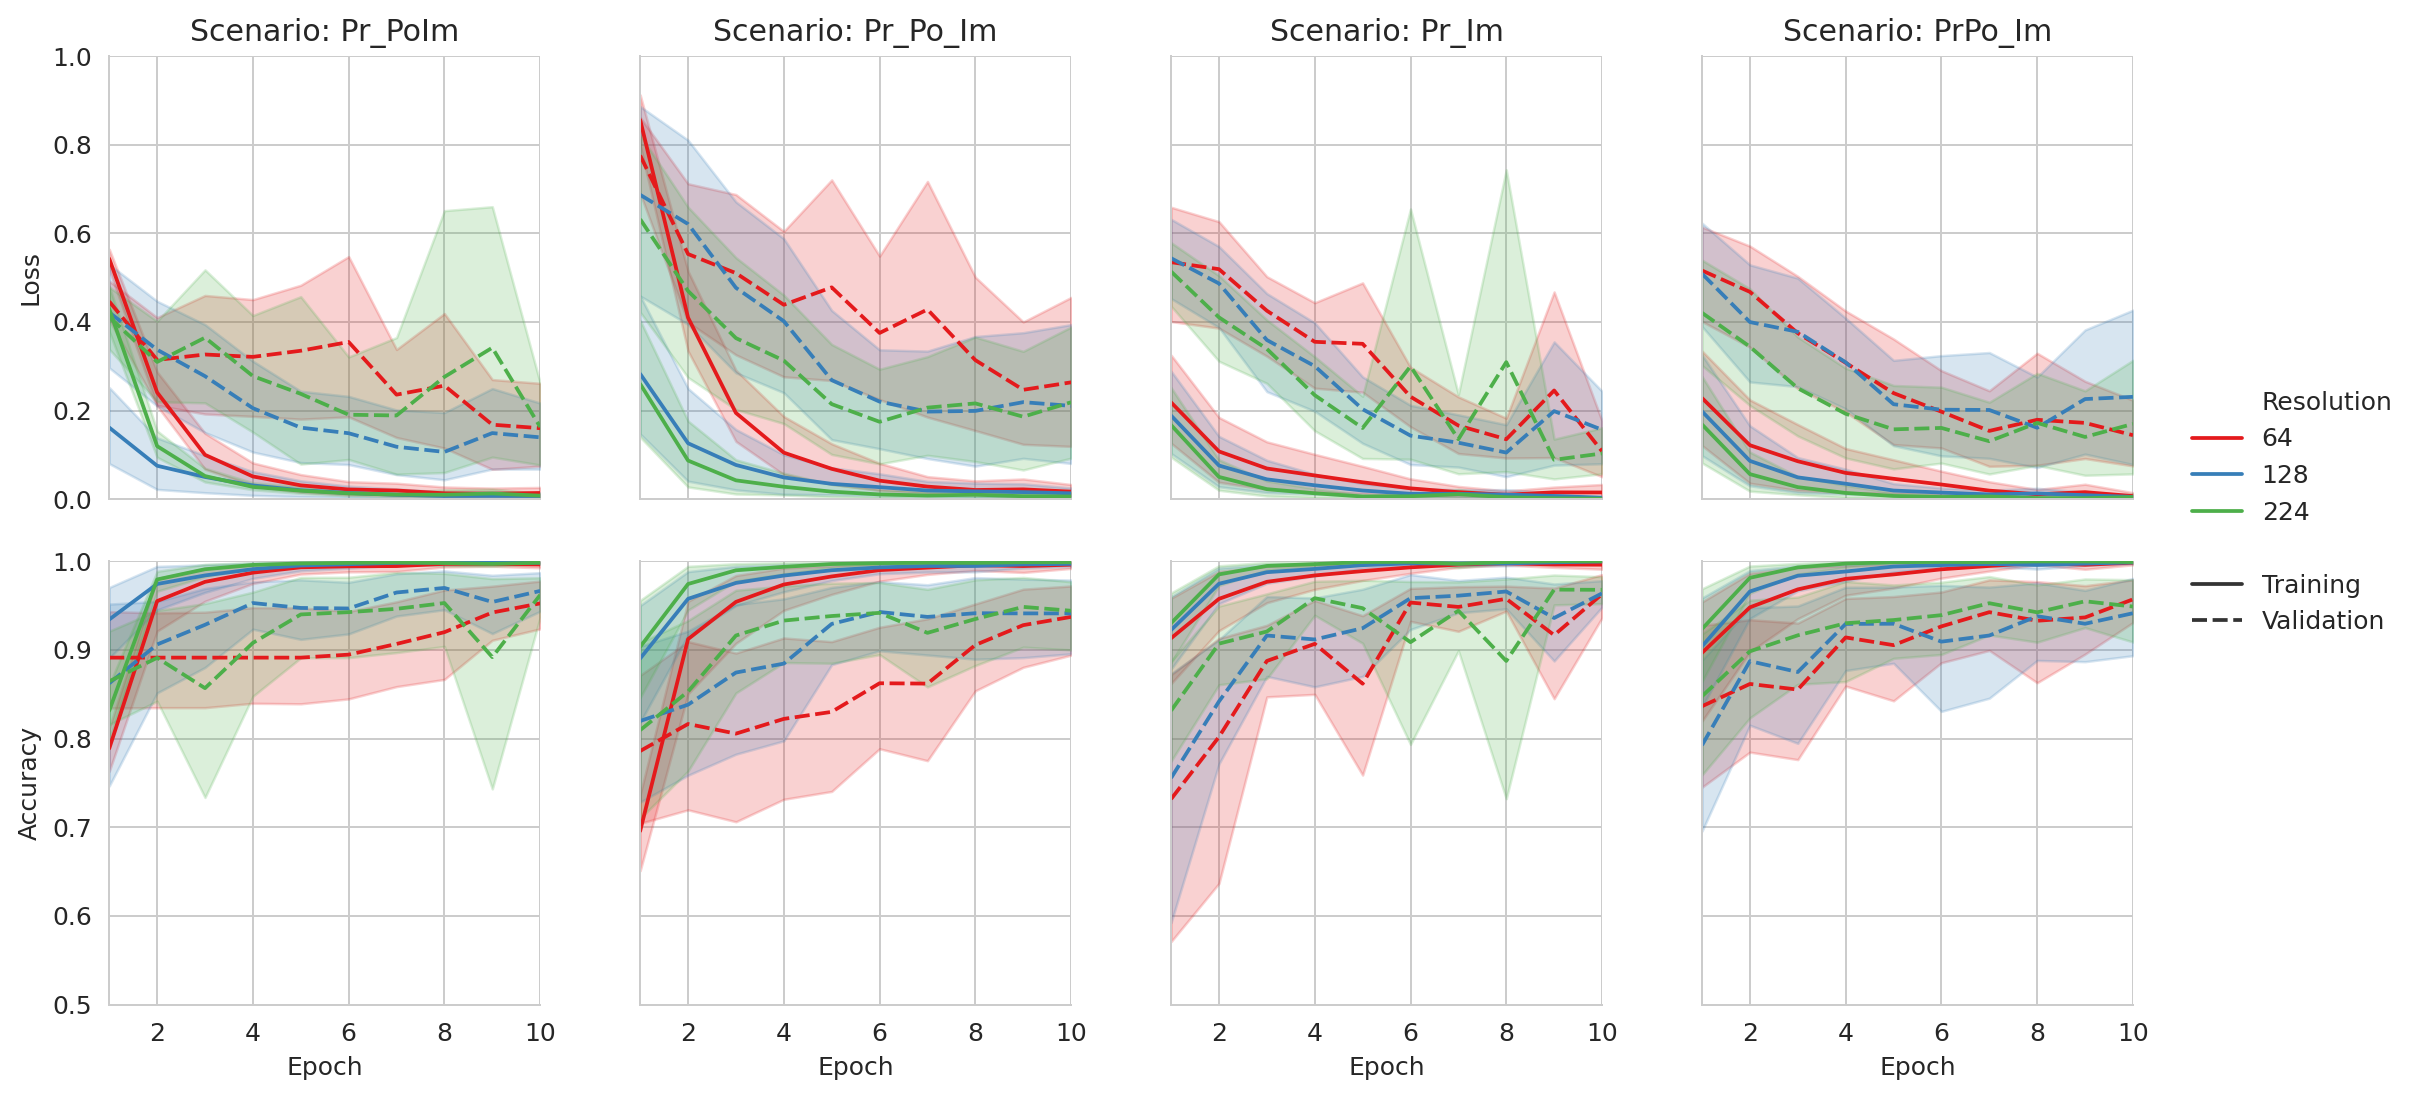
\includegraphics[width=1.05\textwidth]{scenario_resolution_performance.png}
    \caption{Performance metrics for each scenario and input resolution instance. Average metrics and 95\% confidence intervals (trials, $n=5$) are shown for 20 epochs in each case.}
    \label{fig:sens-overall}
\end{figure}

\subsection{Sensitivity to training resolution}
\autoref{fig:sens-val-acc} shows the boxplots of the validation performance metrics for all twelve cases considered.
The metrics are: accuracy and the macro-averages of precision, recall and the $F_{1}$ score.
For reference, we summarize the statistics (mean and standard deviation) of the validation performance metrics in \autoref{tab:meanstd}.
%With respect to the accuracy, there are no significant differences between the 
Taking all metrics into consideration, Welch's pairwise tests show that there are no significant differences in performance among the 3 training resolutions, with one exception.
In the scenario Pr\_PoIm, the accuracy, $F_{1}^{m}$, and $Re^{m}$ for the 128-pixel case are greater than those for the 224-pixel case ($p<.001$).
This difference in performance is not as stark between the 128-pixel and 64-pixel cases in the same scenario.
This outcome implies that we can achieve efficiency by  training at lower resolutions without significant losses in performance.
(A complete summary of the p-values is provided in \autoref{tab:welch-resolution}.)
% Using the Welch test for pairwise comparisons of resolution performance within each scenario, we found no statistically significant difference between the validation accuracy for each resolution ($p\ge 0.57$).

\begin{figure}[ht!]
    \centering
    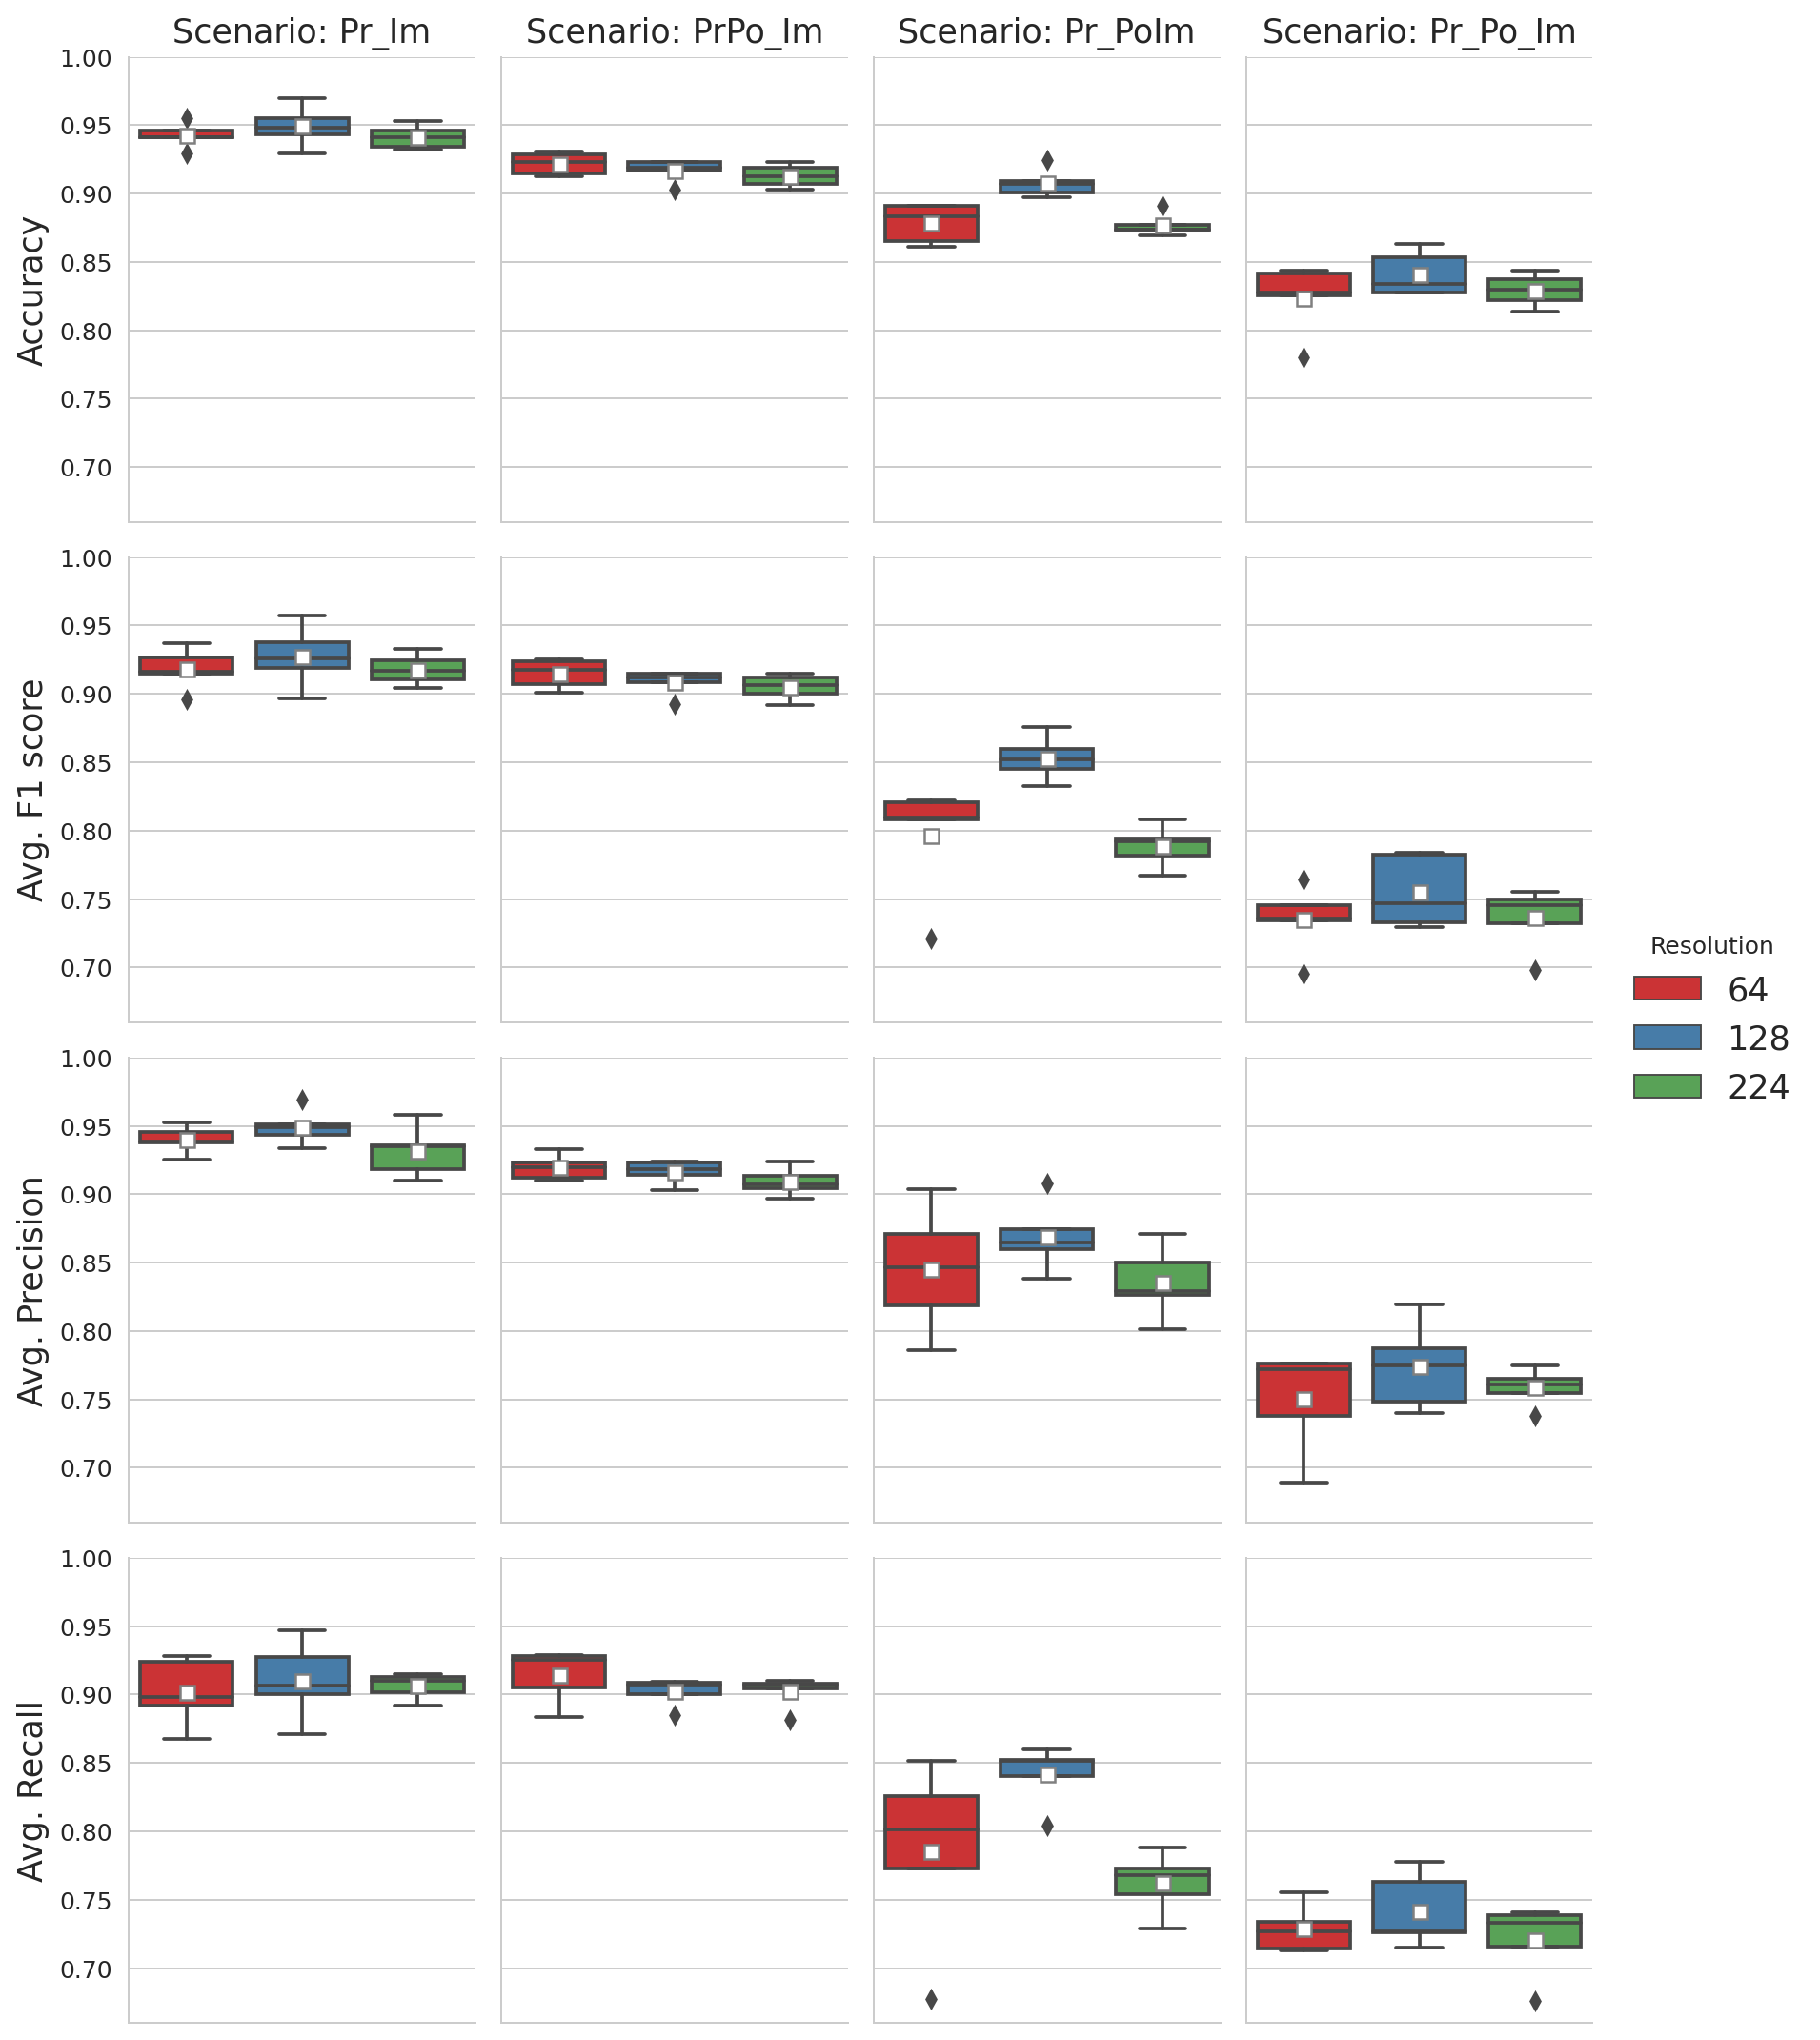
\includegraphics[width=\textwidth]{figures/scenario_resolution_performance_metrics_facet_boxplot.png}
    \caption{Boxplots of validation performance metrics for each scenario and resolution combination.
      The upper and lower bounds of each box are the first and third quartiles; the whiskers are three standard deviations apart; and the diamonds are outliers. Mean values are depicted as white squares in each box.}
 \label{fig:sens-val-acc}
\end{figure}
% \begin{table}[h!]\small
%     \centering
%     \begin{tabular}{ l c r r}\toprule
% \bf Scenario & \bf Resolution & \multicolumn{2}{c}{\bf Validation Accuracy}\\
% & & Mean & SD \\\midrule
%     \texttt{PrPo\_Im} & 64  & 0.96 & 0.04 \\
%                       & 128 & 0.96 & 0.05 \\
%                       &224  &      0.96&  0.05  \\ \midrule        
%     \texttt{Pr\_Im}   & 64  & 0.98 & 0.03 \\
%                       & 128 & 0.97 & 0.03 \\
%                       & 224 & 0.97 & 0.03\\\midrule       
%     \texttt{Pr\_PoIm} & 64  & 0.96 & 0.04 \\
%                       & 128 & 0.97 & 0.04 \\
%                       & 224 & 0.97 & 0.04 \\\midrule       
%     \texttt{Pr\_Po\_Im}& 64  & 0.94 & 0.07 \\
%                       & 128 & 0.95 & 0.07 \\
%                       & 224 & 0.95 & 0.06 \\\bottomrule
%     \end{tabular}
%     \caption{Summary validation accuracy (mean and standard deviation to 2 decimal places) for each scenario and input image resolution training instance. There is no statistically significant difference between the performance for each resolution case under each scenario.}
%     \label{tab:meanvalacc}
% \end{table}

\subsection{Scenario sensitivity}
We conducted pairwise tests between each scenario combination for all resolutions. (A complete summary of the results is given in \autoref{tab:welch-scenario}.
The results indicated that considering all metrics, the scenarios are statistically significantly different from each other ($p < .005$) except Pr\_Im compared to PrPo\_Im and Pr\_PoIm compared to Pr\_Po\_Im, with respect to certain metrics.
If the accuracy is not taken into account, then there is no strong evidence that Pr\_Im differs in performance when compared with PrPo\_Im.
In the case of Pr\_PoIm versus Pr\_Po\_Im, there is greater evidence to support their similarity in performance 
with respect to  $F_{1}^{m}$ and $Re^{m}$. %and $Pr^{m}$
Otherwise, the performance between these two scenarios is significantly different.
From \autoref{fig:sens-val-acc}, we observe the best performances in Pr\_Im and PrPo\_Im, with all metrics greater than or equal to 0.90.
The performance in Pr\_PoIm is lower, and Pr\_Po\_Im has the lowest performance of all four.


Scenario Pr\_Im unsurprisingly has the best performance (greatest accuracy and $Pr^{m}$ of 0.95), since the
classifier only has to predict two extreme categories of \textit{Probable} and \textit{Improbable}.  However, the
\textit{Possible} category cannot be evaded in reality.  Thus, from the perspective of practical application, scenario
PrPo\_Im, which is the next best performing scenario (best accuracy of 0.92, $\hat\sigma=0.01$), demonstrates that it is
most viable to group \textit{Probable} with \textit{Possible} for the best CNN performance.

 
\subsection{Analysis of classification strategies}
Given that there was no significant difference in performance among the three resolutions tested, we focused 
on the 128-px case, as a tradeoff between efficiency and performance. We re-trained the model on all four
scenarios using this resolution and then evaluated performance on the aforementioned validation metrics: accuracy and the macro-averages of
class-specific precision, recall and $F_{1}$ score.
The goal of this analysis was to explore the efficiencies of various classification strategies for tree failure risk.

Using a randomly sampled validation set that was 20\% of the augmented dataset as before, we trained the CNN with the
respective optimal hyperparameters for a single instance in order to compare the performance across the scenarios. The
metrics are shown in \autoref{fig:cnn-perf}.  In each scenario, we trained the model over 13 epochs. % but we employed
% early stopping using validation loss as the criterion with a patience of 3.
% That is, the training routine would set the
% weights of the final model at the epoch from which there was no further improvement in validation loss after three
% subsequent iterations.
From this figure, we see that Pr\_Po\_Im performed significantly worse than the other three. This indicates the
uncertainty surrounding the expert, yet subjective, failure likelihood assessment of the trees to begin
with, particularly when the category is deemed to be \textit{Possible}. % Given the results
% from the sensitivity tests, however, it is possible that a different training instance may have provided better
% results, or perhaps, further iterations were required to achieve convergence.

\begin{figure}[ht]
    \centering
    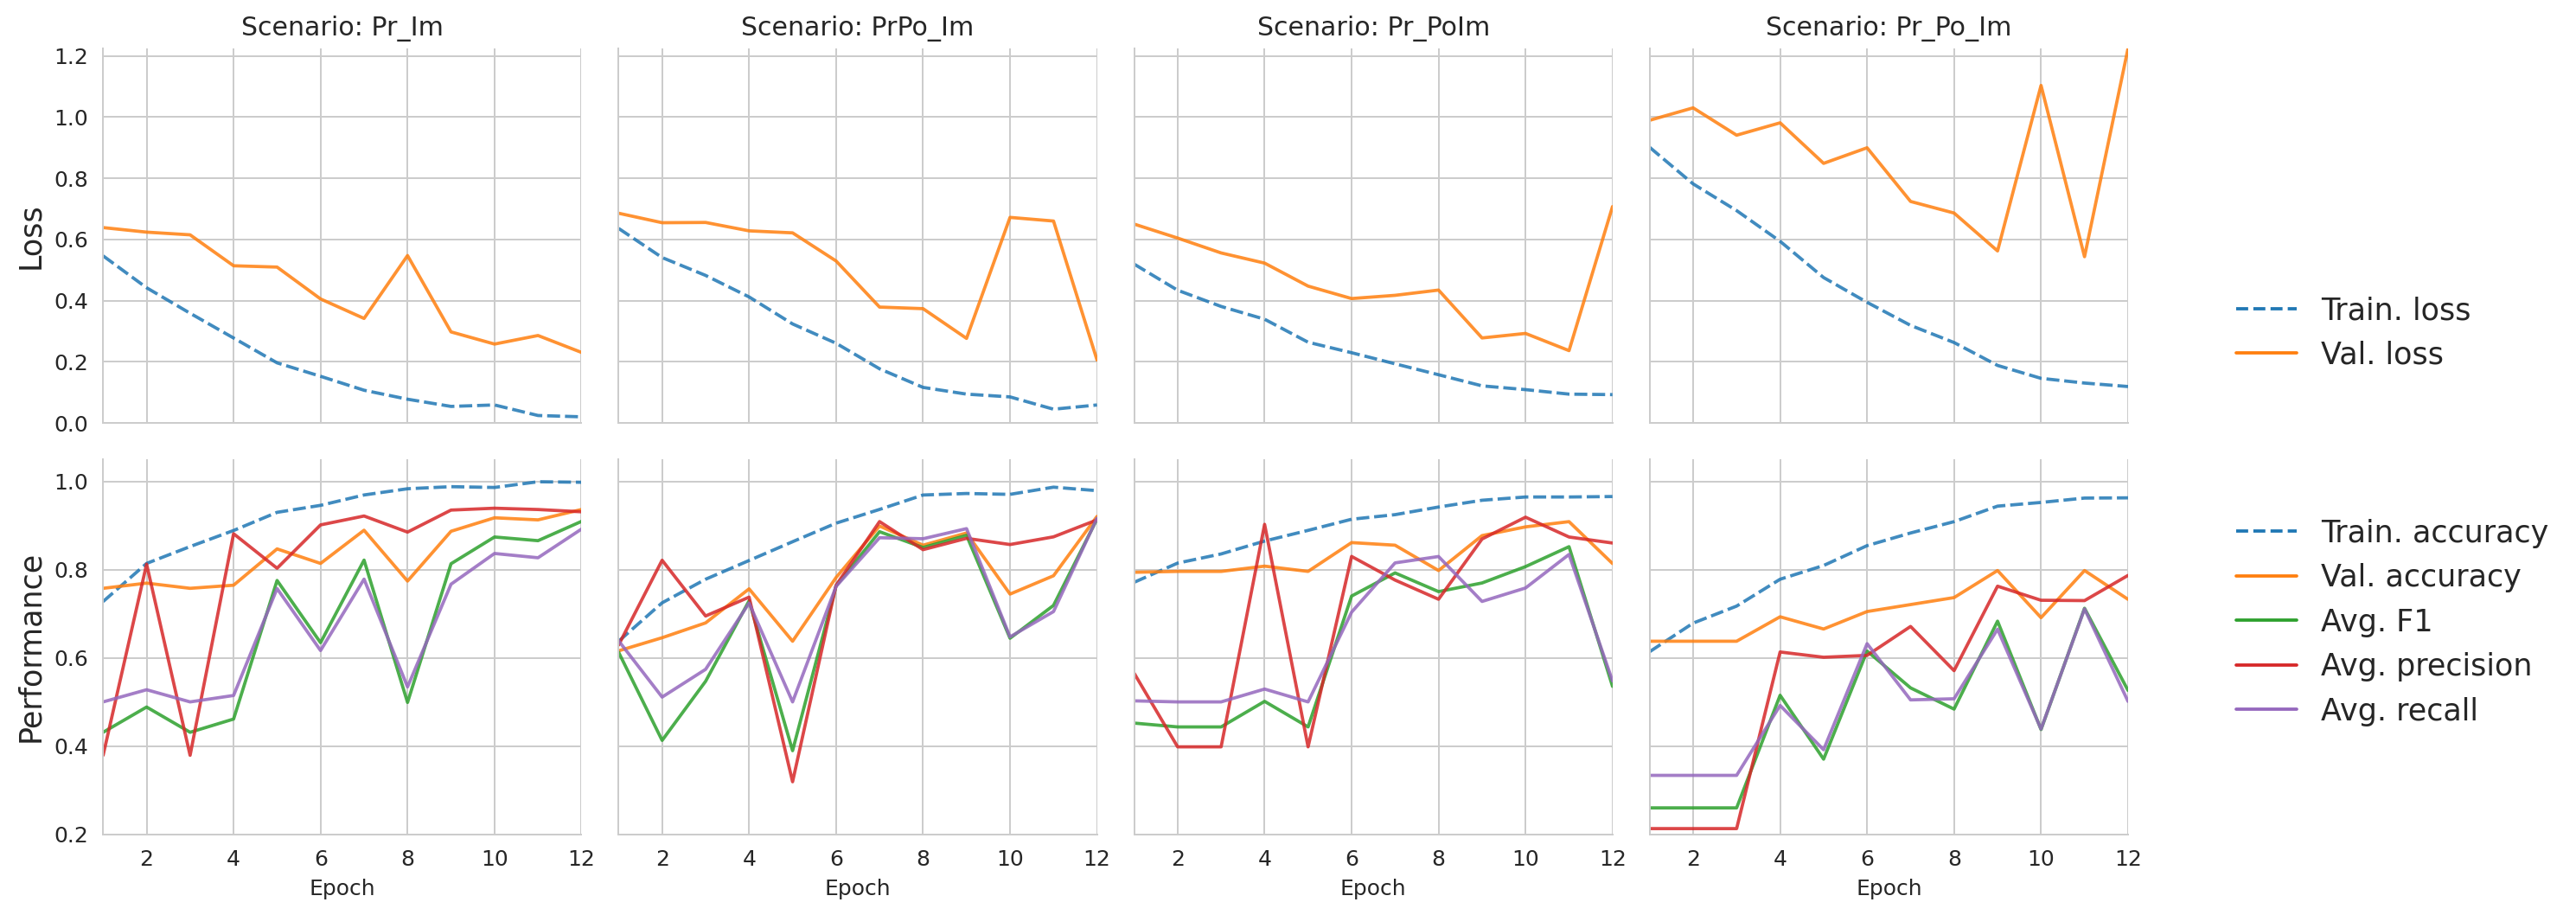
\includegraphics[width=1.05\textwidth]{cnn-performance-metrics-128px-plot}
    \caption{Model performance across four classification scenarios for a single training instance in each case. Training resolution was 128px. All weighted average metrics were computed on the validation set.}
    \label{fig:cnn-perf}
\end{figure}

We also plotted the confusion matrix for each scenario in \autoref{fig:confusion-matrix} to further investigate the
performance of the classifier.  Each row of the confusion matrix indicates the proportion of observations in a given
class that are predicted to be in the classes across the columns.  Thus, the diagonal entry in each matrix represents
the class-specific recall score, $Re_{c}$.  The matrices show that generally, the \textit{Possible} category is
difficult to predict accurately as an individual class.  The classifier performs best when it only has to distinguish
between \textit{Probable} and \textit{Improbable} (\autoref{pr_im_cm}). This observation aligns with previous work \cite{koeser2020can} and is arboriculturally intuitive. The \textit{Improbable} category includes trees with no apparent structural defects, which is comparatively easy for a qualified arborist to assess. When a defect is present, however, an arborist must estimate the severity of the defect that is present, whether the tree has grown in such a way that structurally compensates for the presence of the defect, and the anticipated loads on the tree. Although there are guidelines to inform an arborist's assessment \cite{smiley2017best,goodfellow2020best}, evaluating each of these factors still depends on an arborist's judgment and experience, making it more difficult to distinguish between trees in the \textit{Possible} and \textit{Probable} categories. Thus, it was not surprising that performance only suffered slightly when
\textit{Possible} was grouped with \textit{Probable} in the PrPo\_Im scenario (\autoref{prpo_im_cm}), which we would
select as the best strategy from a practical standpoint.  These two scenarios (Pr\_Im and PrPo\_Im) have the highest
class-specific recall scores $Re_{c}$ ($\ge 0.90$) compared to the other two scenarios Pr\_PoIm ($Re_{c} \ge 0.58$) and
Pr\_Po\_Im ($Re_{c} \ge 0.54)$. In scenario Pr\_PoIm, we see that even grouping \textit{Possible} with
\textit{Improbable} worsens the ability of the classifier to distinguish the \textit{Probable} category.

\begin{figure}[ht]
  \centering
  \begin{subfigure}[t]{.45\linewidth}
    \centering
    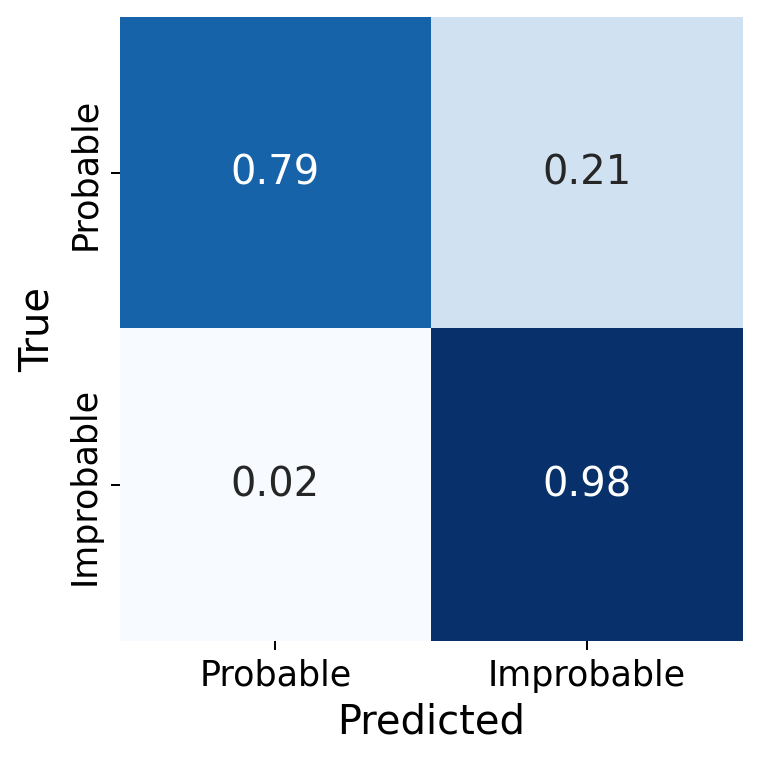
\includegraphics[width=\linewidth, trim={0 0 1cm 1cm}, clip]{opt-confusion-matrix-Pr_Im-128-px.png}
    \caption{Scenario \texttt{Pr\_Im}}
    \label{pr_im_cm}
  \end{subfigure}%
   \begin{subfigure}[t]{.45\linewidth}
    \centering
    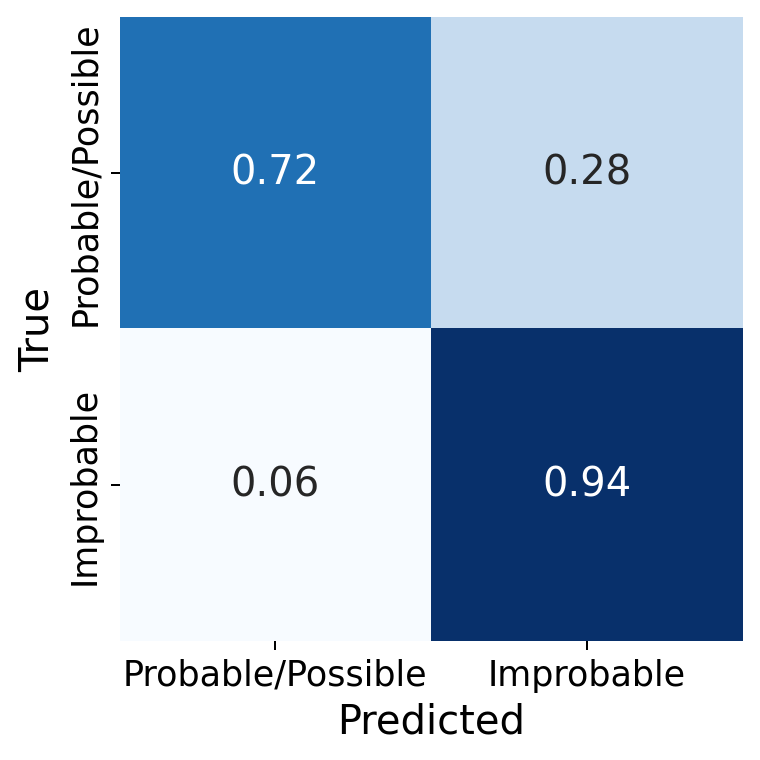
\includegraphics[width=\linewidth, trim={0 0 1cm 1cm}, clip]{opt-confusion-matrix-PrPo_Im-128-px.png}
    \caption{Scenario \texttt{PrPo\_Im}}
    \label{prpo_im_cm}
  \end{subfigure}%
  
  \begin{subfigure}[t]{.45\linewidth}
    \centering
    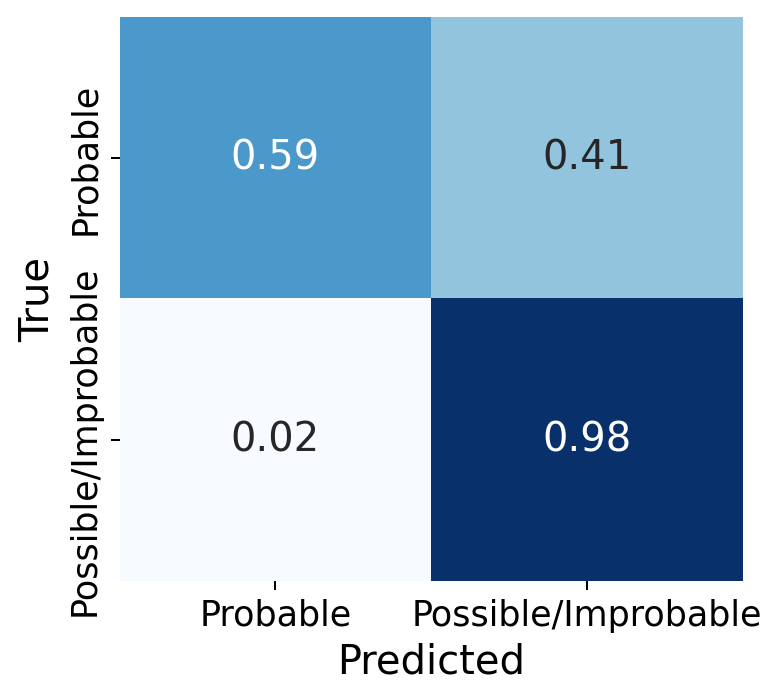
\includegraphics[width=\linewidth, trim={0 0 1cm 1cm}, clip]{opt-confusion-matrix-Pr_PoIm-128-px.png}
    \caption{Scenario \texttt{Pr\_PoIm}}
    \label{pr_poim_cm}
\end{subfigure}%
  \begin{subfigure}[t]{.45\linewidth}
    \centering
    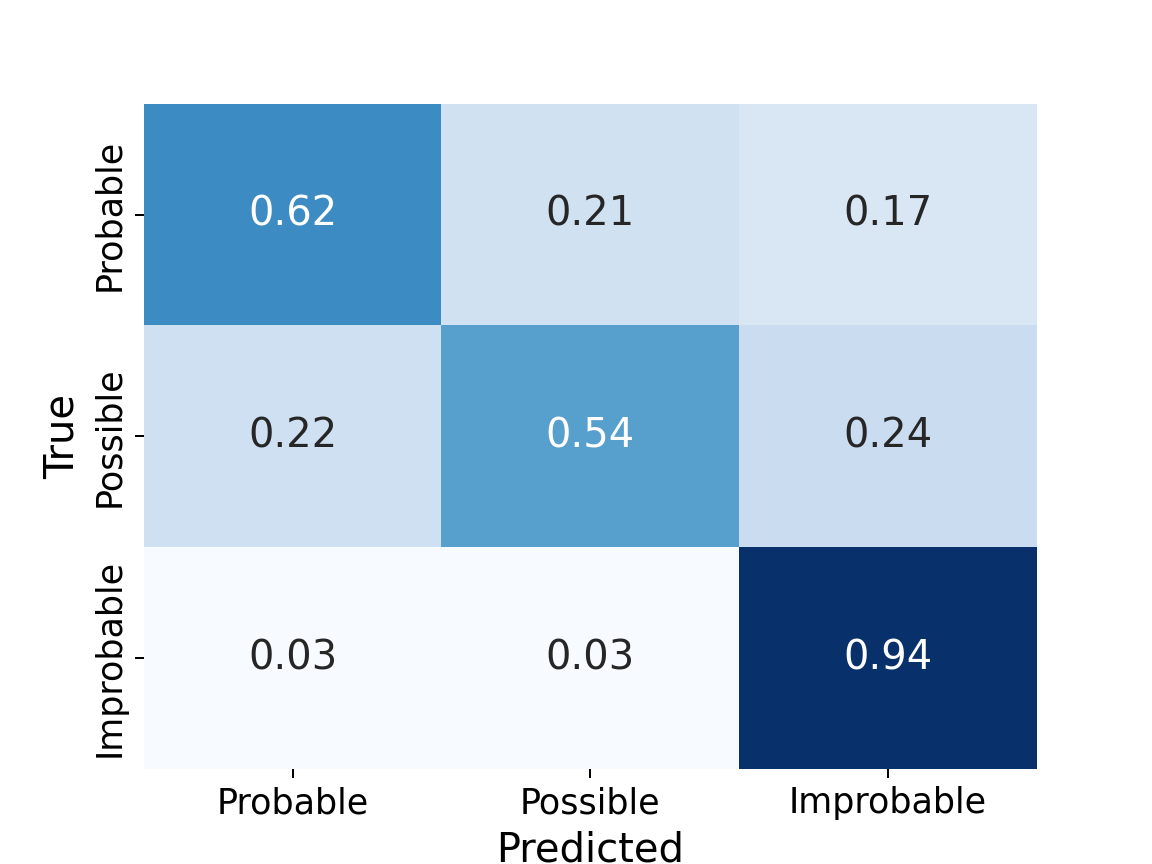
\includegraphics[width=\linewidth, trim={0 0 1cm 1cm}, clip]{opt-confusion-matrix-Pr_Po_Im-128-px.png}
    \caption{Scenario \texttt{Pr\_Po\_Im}}
    \label{pr_po_im_cm}
  \end{subfigure}%
  \caption{Scenario confusion matrices for a single training instance using the 128-pixel images.  Each row of a
    confusion matrix indicates the proportional distribution of class predictions for the true members of each
    class. Thus, the diagonals indicate the recall for each class $Re_c$. The average of the diagonal values gives the
    macro-average $Re^m$ for each scenario.}
    \label{fig:confusion-matrix}
  \end{figure}

%   The detailed performance metrics for the 128-pixel case are summarized in \autoref{tab:performance}.
  
% \begin{table}[ht]\small
%     \centering
% \begin{tabular}{@{}llllll@{}}
% \toprule
% \textbf{Scenario} & \textbf{Averaging method} & \textbf{Precision} & \textbf{Recall} & \textbf{F1-score} & \textbf{Support} \\ \midrule
% Pr\_Im    & Probable            & 0.9  & 0.75 & 0.81 & 103 \\
%          & Improbable          & 0.92 & 0.97 & 0.95 & 322 \\
%          & accuracy            &      &      & 0.92 & 425 \\
%          & weighted avg        & 0.92 & 0.92 & 0.92 & 425 \\ \midrule
% Pr\_Po\_Im & Probable            & 0.82 & 0.56 & 0.67 & 103 \\
%          & Possible            & 0.43 & 0.74 & 0.54 & 80  \\
%          & Improbable          & 0.93 & 0.86 & 0.89 & 322 \\
%          & accuracy            &      &      & 0.78 & 505 \\
%          & weighted avg        & 0.83 & 0.78 & 0.79 & 505 \\ \midrule
% Pr\_PoIm  & Probable            & 0.77 & 0.75 & 0.76 & 103 \\
%          & Possible/Improbable & 0.94 & 0.94 & 0.94 & 402 \\
%          & accuracy            &      &      & 0.9  & 505 \\
%          & weighted avg        & 0.9  & 0.9  & 0.9  & 505 \\ \midrule
% PrPo\_Im  & Probable/Possible   & 0.85 & 0.96 & 0.9  & 183 \\
%          & Improbable          & 0.97 & 0.9  & 0.94 & 322 \\
%          & accuracy            &      &      & 0.92 & 505 \\
%          & weighted avg        & 0.93 & 0.92 & 0.92 & 505 \\ \bottomrule
% \end{tabular}
%     \caption{Detailed performance metrics across the four scenarios in the 128-pixel case (single trial)}
%     \label{tab:performance}
% \end{table}


% \subsection{Model visualization and inference}
% Model explainability is increasingly critical in the application of CNNs to an ever-expanding set of problems.

% \begin{figure}[ht]
%     \centering

%     \begin{subfigure}[t]{.45\linewidth}
%     \centering
%     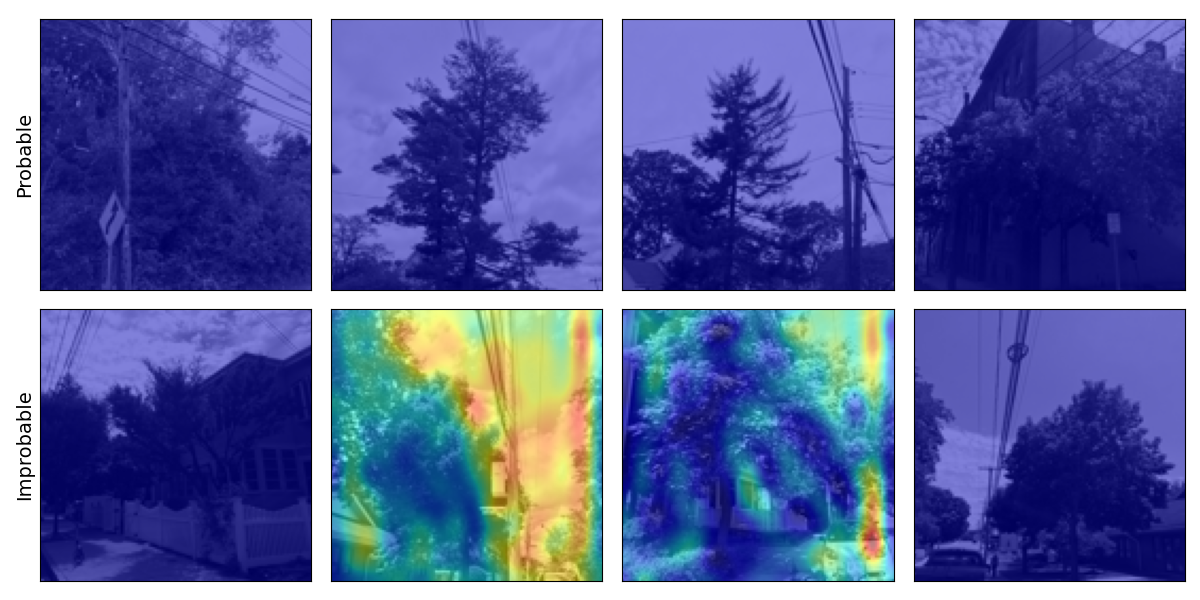
\includegraphics[width=\linewidth]{opt-gradcam-Pr_Im-128-px-4-images.png}
%     \caption{Scenario \texttt{Pr\_Im}}
%     \label{prpo_im_cm}
%     \end{subfigure}%   
%     \begin{subfigure}[t]{.45\linewidth}
%     \centering
%     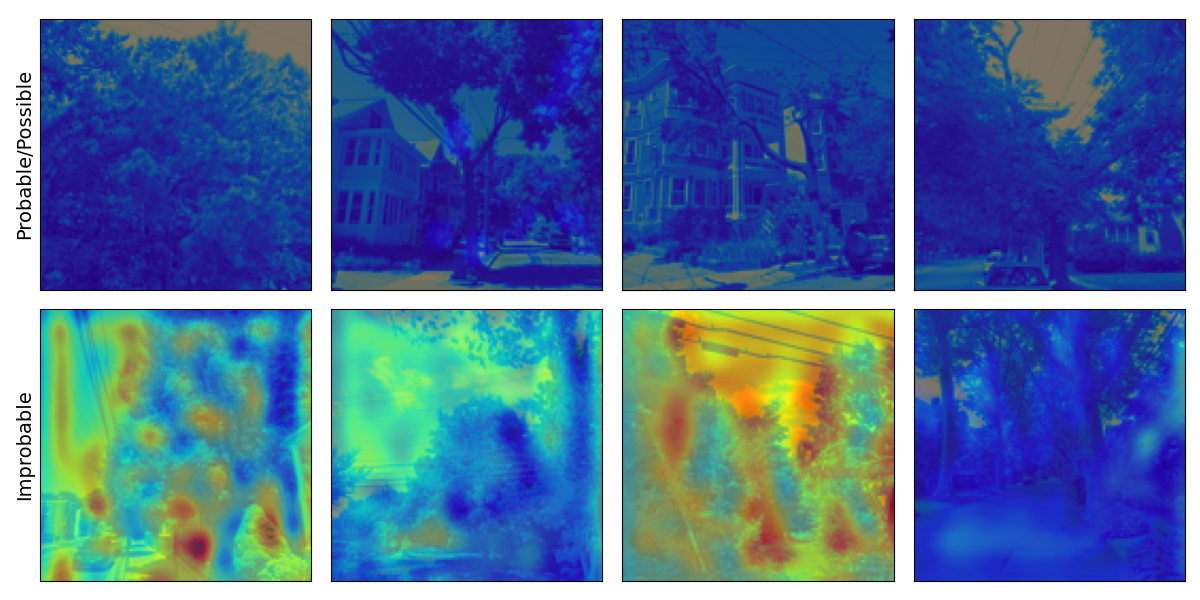
\includegraphics[width=\linewidth]{opt-gradcam-PrPo_Im-128-px-4-images.png}
%     \caption{Scenario \texttt{PrPo\_Im}}
%     \label{prpo_im_cm}
%     \end{subfigure}%
    
%     \begin{subfigure}[t]{.45\linewidth}
%     \centering
%     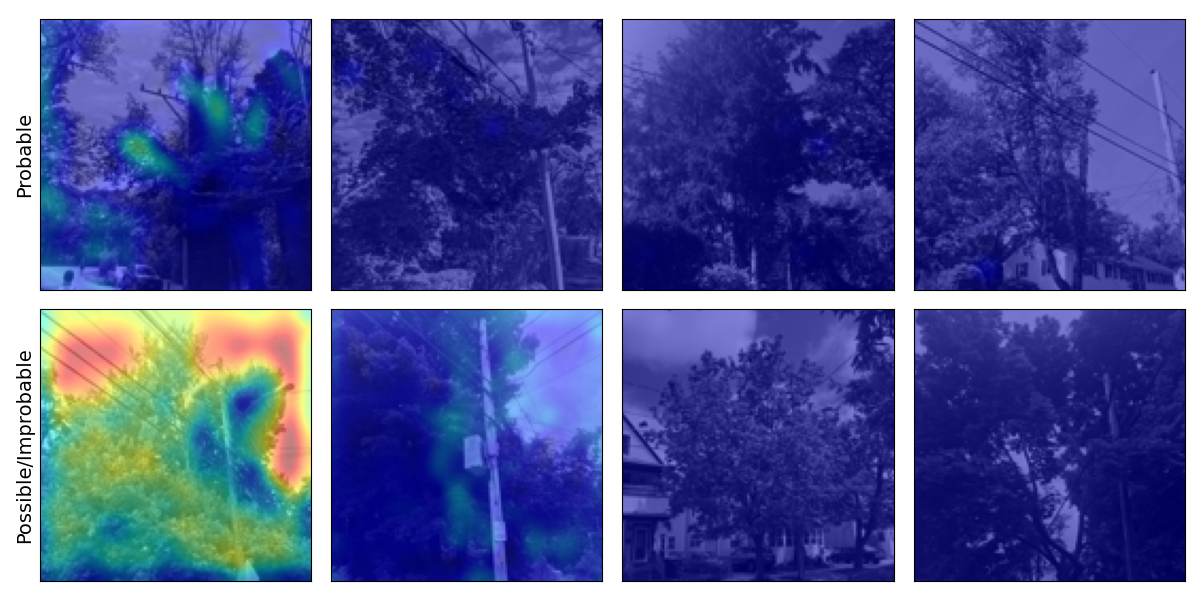
\includegraphics[width=\linewidth]{opt-gradcam-Pr_PoIm-128-px-4-images.png}
%     \caption{Scenario \texttt{Pr\_PoIm}}
%     \label{prpo_im_cm}
%     \end{subfigure}%
%     \begin{subfigure}[t]{.45\linewidth}
%     \centering
%     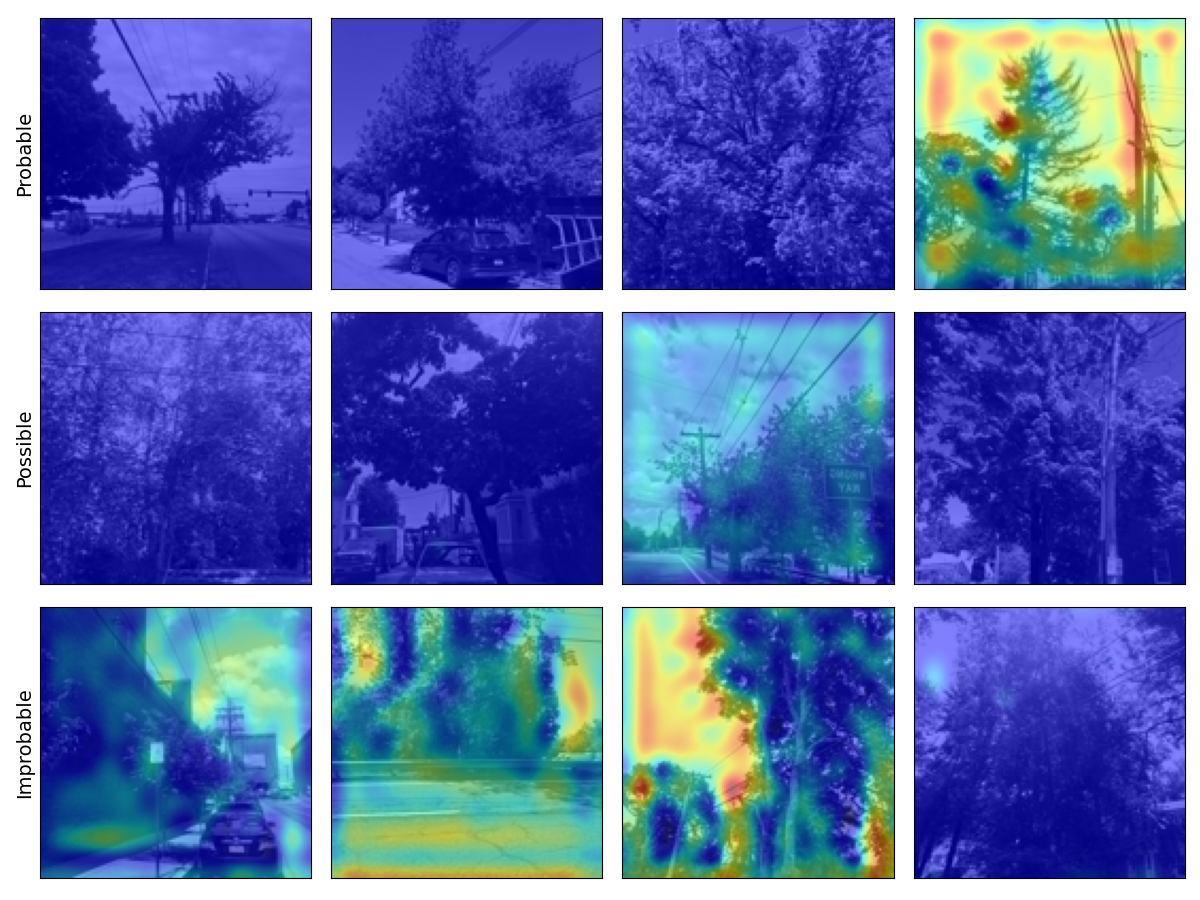
\includegraphics[width=\linewidth]{opt-gradcam-Pr_Po_Im-128-px-4-images.png}
%     \caption{Scenario \texttt{Pr\_Po\_Im}}
%     \label{prpo_im_cm}
%     \end{subfigure}%
    
%     \caption{Gradient-weighted class activation maps (Grad-CAMs) for randomly selected validation images in each class. (Resolution: 128px)}
%     \label{fig:my_label}
% \end{figure}

% \subsection{Comparison with state-of-the-art architectures}
% We compare the performance of our selected model with existing high-performance architectures. The results are summarized in \autoref{tab:comp}.

% \begin{table}[h!]\small
%   \centering
%   \begin{tabular}{l l l l l l l }\toprule
%     \bf Model & \multicolumn{3}{c}{\bf Training metrics} &\multicolumn{3}{c}{\bf Validation metrics}  \\\midrule
%     & Error & Precision & Recall     & Error & Precision & Recall \\
%     SafeTree & & & & & & \\
%     GoogleNet (InceptionV3) & & & & & & \\
%     ResNet50 & & & & & & \\
%         VGGNet & & & & & & \\
%     AlexNet & & & & & & \\\bottomrule
%   \end{tabular}
%   \caption{Comparing our model SafeTree with state-of-the-art CNN architectures trained on our data}
%   \label{tab:comp}
% \end{table}

\section{Conclusion}
We have demonstrated the efficacy of an artificial intelligence framework for predicting tree failure likelihood
(\textit{Probable}, \textit{Possible} and \textit{Improbable}) with respect to utility infrastructure. Specifically, we
developed a convolutional neural network with state-of-the-art configurations.  We applied data augmentation and
pre-processing strategies to increase the size of our dataset by a factor of 5, thus generating 2525 images.  From an
initial resolution of $4032 \times 3024$ pixels, we created three sets of image resolutions: $64 \times 64$,
$128 \times 128$ and $224 \times 224$. We then defined four classification scenarios to investigate the performance of
various groupings of the three categories: Pr\_Im (\textit{Probable} vs.\ \textit{Improbable}); PrPo\_Im
(\textit{Probable} and \textit{Possible} vs.\ \textit{Improbable}); Pr\_PoIm (\textit{Probable} vs.\ \textit{Possible}
and \textit{Improbable}); and Pr\_Po\_Im (\textit{Probable} vs.\ \textit{Possible} vs. \textit{Improbable}).
We then optimized eight of our CNN hyperparameters for 12 classification
scenario and image resolution combinations.  We conducted five-fold cross-validation for each of the 12 cases, and
assessed model performance based on accuracy and the macro-averages of precision, recall and $F_{1}$ score.

Our results indicated that there generally was no significant difference in performance between the resolutions.  Among
the scenarios, however, Pr\_Im performed the best with a top accuracy and $Pr^{m}$ of 0.94 ($\hat\sigma = 0.01)$.
The next best-performing scenario was PrPo\_Im with a top accuracy and $Pr^{m}$ of 0.92 ($\hat\sigma = 0.01$).  For
practical applications, scenario PrPo\_Im is more realistic, as it includes all three categories.  Thus, we deemed this
as the most viable.  Scenarios Pr\_PoIm and Pr\_Po\_Im had best accuracy scores of 0.91 ($\hat\sigma = 0.01$) and 0.84
($\hat\sigma = 0.02$), respectively.  But their performance across the other metrics was considerably worse.

We further conducted more detailed classification performance analyses over single training instances for the 128-pixel
case.  Our results indicate that the CNN performed best at recalling \textit{Probable} vs. \textit{Improbable} or
\textit{Probable}/\textit{Possible} vs.\ \textit{Improbable}.  The \textit{Possible} category appeared to be a
confounding for the classifier.  This was not unexpected, given the uncertainty and subjectivity in assessing these trees
to begin with.  The CNN, however, performed better at distinguishing between \textit{Possible}/\textit{Improbable} and
\textit{Probable}, than between \textit{Probable}/\textit{Possible} and \textit{Improbable}.  This might be an indicator
that trees in the \textit{Possible} category are more likely to be identified as \textit{Improbable}.  When all three
failure-likelihood categories were predicted individually in scenario Pr\_Po\_Im, the \textit{Possible} category had the
lowest class-specific recall score.

Nevertheless, given the relatively small input dataset of original images, these preliminary results are extremely
promising for future improvements.  First, we can train better models with more data.  We also plan to rigorously
quantify the uncertainty in ground truth category assignments by incorporating predictions from multiple experts on the
same images.  In order to better understand how the CNN is classifying each image, we will conduct extensive visual
inference in further work, for instance, using the gradient-weighted class activation mapping approach
\cite{zeiler2014visualizing}.  There is also a potential for mapping the visual cues learned by the CNN to physical
relationships governing tree structure, in order to gain greater insights into tree failure processes.  The automation
for tree failure likelihood assessments can potentially supplement human decision-making for increased resilience and,
in the future, reduce costs and improve reliability in tree assessments, thus leading to more sustainable communities.


\section{Data Availability Statement}
All data, models, or code generated or used during the study are publicly available in a GitHub repository online at \url{https://github.com/narslab/tree-risk-ai}.

\section{Acknowledgments}
The authors acknowledge the partial support of Eversource Energy in funding this work.

\appendix
\section{Summary of validation performance metrics}
For further reference we tabulate the mean and standard deviation of the performance metrics obtained on the scenario-resolution sensitivity tests. These values are shown in \autoref{tab:meanstd}.
The metrics are: accuracy, macro-average $F_1$ ($F_1^m$), macro-average recall ($Re^m$) and macro-average precision ($Pr^m$).

\begin{table}[ht]\small\centering
\caption{Mean and standard deviation of the 5-fold cross-validation estimates of classifier performance metrics on the 12 scenario-resolution cases investigated. ``SD'' represents ``standard deviation.''}
\label{tab:meanstd}
\begin{tabular}{llllllllll}\toprule
\multirow{3}{*}{\textbf{Scenario}} &  
\multirow{3}{*}{\textbf{Resolution}}  & \multicolumn{2}{c}{\textbf{Accuracy}} & \multicolumn{2}{c}{$\bm{F_1^m}$} 
& \multicolumn{2}{c}{$\bm{Re^m}$} & \multicolumn{2}{c}{$\bm{Pr^m}$} \\%\cmidrule{3-10}
                          &            & Mean & SD  & Mean & SD  & Mean & SD  & Mean & SD  \\\midrule
\multirow{3}{*}{Pr\_Im}    & 64        & 0.94 & 0.01 & 0.92 & 0.02 & 0.9  & 0.02 & 0.94 & 0.01 \\
                          & 128        & 0.95 & 0.01 & 0.93 & 0.02 & 0.91 & 0.03 & 0.95 & 0.01 \\
                          & 224        & 0.94 & 0.01 & 0.92 & 0.01 & 0.91 & 0.01 & 0.93 & 0.02 \\\midrule
\multirow{3}{*}{PrPo\_Im}  & 64         & 0.92 & 0.01 & 0.91 & 0.01 & 0.91 & 0.02 & 0.92 & 0.01 \\
                          & 128        & 0.92 & 0.01 & 0.91 & 0.01 & 0.9  & 0.01 & 0.92 & 0.01 \\
                          & 224        & 0.91 & 0.01 & 0.91 & 0.01 & 0.9  & 0.01 & 0.91 & 0.01 \\\midrule
\multirow{3}{*}{Pr\_PoIm}  & 64         & 0.88 & 0.01 & 0.8  & 0.04 & 0.79 & 0.07 & 0.85 & 0.05 \\
                          & 128        & 0.91 & 0.01 & 0.85 & 0.02 & 0.84 & 0.02 & 0.87 & 0.03 \\
                          & 224        & 0.88 & 0.01 & 0.79 & 0.02 & 0.76 & 0.02 & 0.84 & 0.03 \\\midrule
\multirow{3}{*}{Pr\_Po\_Im} & 64         & 0.82 & 0.03 & 0.74 & 0.03 & 0.73 & 0.02 & 0.75 & 0.04 \\
                          & 128        & 0.84 & 0.02 & 0.76 & 0.03 & 0.74 & 0.03 & 0.77 & 0.03 \\
                          & 224        & 0.83 & 0.01 & 0.74 & 0.02 & 0.72 & 0.03 & 0.76 & 0.01\\ \bottomrule
\end{tabular}
\end{table}

\section{Welch $t$-test results}
Here, we summarize the p-values resulting from the Welch independent $t$-tests used to determine if the mean values of the various performance metrics are statistically significant or not.
Strong evidence of significant difference is given by a low p-value (a typical threshold is $< 0.01$).
In \autoref{tab:welch-resolution}, we consider pairwise comparisons between different image resolutions in all four scenarios.
In \autoref{tab:welch-scenario}, we compare different scenarios for the same image resolution.

\begin{table}[ht]\small\centering
\caption{Welch's $t$-test p-value results for pairwise comparisons between image resolutions across all four scenarios.
Low p-values indicates statistically different mean values for the validation metrics considered.}
\label{tab:welch-resolution}
\sisetup{scientific-notation=true, round-precision = 3,round-mode=figures,table-format = 1.2e-1,
exponent-product=\ensuremath{\cdot}}%output-exponent-marker = \text{e}, 
\begin{tabular}{@{}lll SSSS@{}}
\toprule
\multirow{2}{*}{\textbf{Scenario}} &
\multirow{2}{*}{\textbf{Resolution 1}} &
\multirow{2}{*}{\textbf{Resolution 2}} &
\multicolumn{4}{c}{\textbf{p-values}} \\ %\cmidrule(l){4-7} 
    & & & 
  \multicolumn{1}{c}{\textbf{Accuracy}} &
  \multicolumn{1}{c}{$\bm{F_1^m}$} &
  \multicolumn{1}{c}{$\bm{Re^m}$} &
  \multicolumn{1}{r}{$\bm{Pr^m}$} \\ \midrule
\multirow{3}{*}{Pr\_Im}    & 64  & 128 & 0.427766 & 0.472000 & 0.638283 & 0.243409 \\
                          & 64  & 224 & 0.810526 & 0.957770 & 0.728743 & 0.400994 \\
                          & 128 & 224 & 0.333005 & 0.421449 & 0.781772 & 0.119129 \\\midrule
\multirow{3}{*}{PrPo\_Im}  & 64  & 128 & 0.343214 & 0.334622 & 0.280111 & 0.607451 \\
                          & 64  & 224 & 0.112543 & 0.153209 & 0.299562 & 0.131835 \\
                          & 128 & 224 & 0.465132 & 0.566733 & 0.978346 & 0.253573 \\\midrule
\multirow{3}{*}{Pr\_PoIm}  & 64  & 128 & 0.006932 & 0.037836 & 0.139458 & 0.345129 \\
                          & 64  & 224 & 0.836653 & 0.715576 & 0.494841 & 0.697297 \\
                          & 128 & 224 & 0.001099 & 0.000207 & 0.000467 & 0.076234 \\\midrule
\multirow{3}{*}{Pr\_Po\_Im} & 64  & 128 & 0.241587 & 0.249616 & 0.391389 & 0.311935 \\
                          & 64  & 224 & 0.677163 & 0.937617 & 0.598361 & 0.650331 \\
                          & 128 & 224 & 0.227783 & 0.258068 & 0.252791 & 0.366722 \\ \bottomrule
\end{tabular}
\end{table}

% Please add the following required packages to your document preamble:
% \usepackage{booktabs}
% \usepackage{multirow}
\begin{table}[ht]\small\centering
\caption{Welch's $t$-test p-value results for pairwise comparisons between scenarios resolutions for all three image resolutions.
Low p-values indicates statistically different mean values for the validation metrics considered.}
\label{tab:welch-scenario}
\sisetup{scientific-notation=true, round-precision = 3,round-mode=figures,table-format = 1.2e-1,
exponent-product=\ensuremath{\cdot}}%output-exponent-marker = \text{e}, 

\begin{tabular}{@{}lllSSSS@{}}
\toprule
\multirow{2}{*}{\textbf{Scenario}} &
\multirow{2}{*}{\textbf{Resolution 1}} &
\multirow{2}{*}{\textbf{Resolution 2}} &
\multicolumn{4}{c}{\textbf{p-values}} \\ %\cmidrule(l){4-7} 
    & & & 
  \multicolumn{1}{c}{\textbf{Accuracy}} &
  \multicolumn{1}{c}{$\bm{F_1^m}$} &
  \multicolumn{1}{c}{$\bm{Re^m}$} &
  \multicolumn{1}{r}{$\bm{Pr^m}$} \\ \midrule
\multirow{6}{*}{64}  & Pr\_Im   & PrPo\_Im  & 0.005913 & 0.714479 & 0.422914 & 0.010639 \\
                     & Pr\_Im   & Pr\_PoIm  & 0.000068 & 0.001772 & 0.014794 & 0.008354 \\
                     & Pr\_Im   & Pr\_Po\_Im & 0.000184 & 0.000004 & 0.000004 & 0.000193 \\
                     & PrPo\_Im & Pr\_PoIm  & 0.000814 & 0.002534 & 0.010824 & 0.020167 \\
                     & PrPo\_Im & Pr\_Po\_Im & 0.000553 & 0.000014 & 0.000000 & 0.000351 \\
                     & Pr\_PoIm & Pr\_Po\_Im & 0.005380 & 0.029135 & 0.132204 & 0.007418 \\\midrule
\multirow{6}{*}{128} & Pr\_Im   & PrPo\_Im  & 0.004705 & 0.137997 & 0.578580 & 0.002389 \\
                     & Pr\_Im   & Pr\_PoIm  & 0.001249 & 0.000455 & 0.003295 & 0.000790 \\
                     & Pr\_Im   & Pr\_Po\_Im & 0.000005 & 0.000004 & 0.000012 & 0.000060 \\
                     & PrPo\_Im & Pr\_PoIm  & 0.169503 & 0.000446 & 0.001725 & 0.011313 \\
                     & PrPo\_Im & Pr\_Po\_Im & 0.000099 & 0.000064 & 0.000050 & 0.000320 \\
                     & Pr\_PoIm & Pr\_Po\_Im & 0.000132 & 0.000244 & 0.000244 & 0.000931 \\\midrule
\multirow{6}{*}{224} & Pr\_Im   & PrPo\_Im  & 0.000716 & 0.088647 & 0.576529 & 0.055010 \\
                     & Pr\_Im   & Pr\_PoIm  & 0.000002 & 0.000001 & 0.000025 & 0.000256 \\
                     & Pr\_Im   & Pr\_Po\_Im & 0.000000 & 0.000005 & 0.000029 & 0.000000 \\
                     & PrPo\_Im & Pr\_PoIm  & 0.000130 & 0.000003 & 0.000014 & 0.001828 \\
                     & PrPo\_Im & Pr\_Po\_Im & 0.000003 & 0.000014 & 0.000017 & 0.000000 \\
                     & Pr\_PoIm & Pr\_Po\_Im & 0.000144 & 0.003617 & 0.029345 & 0.001147 \\ \bottomrule
\end{tabular}
\end{table}


\eject
\bibliography{ai-trees-references}   



\end{document}

 
%%% Local Variables:
%%% mode: latex
%%% TeX-master: t
%%% End:
